\documentclass[14pt]{article}
\usepackage[top=2cm,bottom=2cm,left=2.5cm,right=2cm]{geometry}
\usepackage[utf8]{vietnam}
\usepackage{amssymb}
\usepackage{graphicx}
\usepackage{url}


\begin{document}
	\tableofcontents % Lệnh này sẽ tạo mục lục
	\newpage
	\section*{Lời Nói Đầu}
	\begin{flushleft}
		Chúng ta đã biết, trong khoảng 10 năm trở lại đây, công nghệ thông tin đã bùng nổ và phát triển mạnh mẽ ở nước ta. Có thể nói sự phát triển như vũ bão của khoa học và công nghệ trong thời gian qua đã tạo ra những sản phẩm công nghệ mới và đem lại rất nhiều lợi ích cho cuộc sống. Nó đang chiếm phần lớn trong việc phục vụ của nhiều ngành nghề cũng như phục vụ đời sống của con người. Cùng với đó là loài người chúng ta luôn muốn tìm hiểu, cải tiến và khắc phục các nhược điểm của các bài toán có trong cuộc sống. Ví dụ như bài toán lập lịch, người bán hàng,... cho nên trong bài báo cáo này em tập trung nghiên cứu về hai thuật toán được áp dụng nhiều để giải quyết các bài toán tối ưu, cùng với đó là so sánh với các thuật toán khác để thấy được sự khác biệt mà hai thuật toán mang lại.
		
		Trân trọng.
	\end{flushleft}

	
	\newpage
	\section{Phần 1: Tổng quan về đề tài}
	\subsection{Giới thiệu}
	\begin{enumerate}

		\item\textbf{Thuật toán mô phỏng tự nhiên:} là nhóm các phương pháp tính toán bắt chước các quy trình và hệ thống tự nhiên để giải quyết các vấn đề trong toán học và khoa học máy tính. Các thuật toán này thường được dùng trong những tình huống mà các phương pháp truyền thống không hiệu quả hoặc quá chậm. Dưới đây là một cái nhìn tổng quan về các đặc điểm chính của các thuật toán mô phỏng tự nhiên:
		\begin{enumerate}
			\item \textbf{Nguyên tắc hoạt động:} Các thuật toán mô phỏng tự nhiên hoạt động dựa trên nguyên tắc của quá trình sinh học, hành vi động vật, hoặc các hiện tượng tự nhiên khác. Chúng sử dụng các quy tắc đơn giản để mô phỏng các quy trình phức tạp, từ đó phát sinh ra các giải pháp tối ưu hoặc gần tối ưu.
			\item \textbf{Ứng dụng:} Các thuật toán này được ứng dụng rộng rãi trong nhiều lĩnh vực như tối ưu hóa, nhận dạng mẫu, xử lý hình ảnh, dự báo thời tiết, phân tích dữ liệu sinh học, và hơn thế nữa. Chúng đặc biệt hữu ích trong các bài toán tối ưu hóa tổ hợp và liên tục mà không gian tìm kiếm quá lớn hoặc phức tạp.
		\end{enumerate}
		

		\item\textbf{Đối tượng nghiên cứu:}	Như đã nói ở trên thì bài báo cáo này của em sẽ nghiên cứu về 2 thuật toán chủ đạo đó là thuật toán di truyền (Genetic Algorithms - GA), thuật toán tối ưu hóa đàn kiến (Ant Colony Optimization - ACO).
		\begin{enumerate}
			\item \textbf{GA (Genetic Algorithms):} Là một thuật toán tối ưu hóa nguồn cảm hứng từ tự nhiên, mô phỏng quá trình tiến hóa sinh học. Thuật toán này sử dụng các cơ chế di truyền như chọn lọc tự nhiên, lai ghép (crossover), và đột biến (mutation) để tạo ra các thế hệ giải pháp mới từ thế hệ hiện tại. GA bắt đầu từ một quần thể các cá thể (các giải pháp) ngẫu nhiên, sau đó lặp đi lặp lại quá trình chọn lọc, lai ghép, và đột biến để cải thiện chất lượng của quần thể. Thuật toán này phù hợp cho các bài toán tối ưu hóa liên tục hoặc tổ hợp, ví dụ như tối ưu hóa thiết kế, tối ưu hóa đa mục tiêu, và vấn đề phân công.
			\item \textbf{ACO (Ant Colony Optimization):} Là một thuật toán tối ưu hóa nguồn cảm hứng từ tự nhiên, dựa trên hành vi tìm kiếm thức ăn của đàn kiến. Thuật toán này được Marco Dorigo đề xuất vào đầu những năm 1990. Trong ACO, các kiến khám phá không gian tìm kiếm và xây dựng các giải pháp dựa trên phép đánh giá chất lượng của các giải pháp và một chất pheromone mà chúng tiết ra. Chất pheromone này giúp hướng dẫn các kiến khác đến các giải pháp tốt hơn. Thuật toán này thường được sử dụng để giải quyết các bài toán tối ưu hóa tổ hợp, chẳng hạn như bài toán người bán hàng (Travelling Salesman Problem - TSP), bài toán lập lịch, và các bài toán tuyến đường.
			\end{enumerate}
	\end{enumerate}
	\subsection{Lý do chọn đề tài}
	\begin{itemize}
		\item \textbf{Ứng dụng Rộng Rãi:} Cả ACO và GA đều có khả năng ứng dụng rộng rãi trong nhiều lĩnh vực khác nhau như tối ưu hóa trong lĩnh vực logistics, lập lịch sản xuất, vận tải, thiết kế mạng, và nhiều bài toán khoa học khác. Việc tìm hiểu sâu về các thuật toán này có thể mở ra nhiều cơ hội áp dụng thực tế.
		\item \textbf{Cải Thiện và Đổi Mới:} Cả hai thuật toán đều cho phép không gian lớn để đổi mới và cải tiến. Có thể tập trung vào cải thiện hiệu quả tính toán của chúng, hoặc phát triển các biến thể mới phù hợp hơn với các loại bài toán cụ thể.
		\item \textbf{Giải quyết Bài toán Phức Tạp:} Thuật toán ACO và GA đặc biệt hữu ích trong việc giải quyết các bài toán tối ưu hóa phức tạp, nơi các phương pháp truyền thống không hiệu quả. Chọn các thuật toán này làm đề tài nghiên cứu có thể giúp giải quyết những thách thức thực tế trong các ngành công nghiệp và nghiên cứu.
		\item \textbf{Nhu cầu Thực Tiễn và Thương Mại:} Cả hai thuật toán có nhiều ứng dụng thực tế có thể chuyển giao sang các sản phẩm và dịch vụ thương mại. Tìm hiểu về chúng có thể cung cấp nền tảng để phát triển các giải pháp công nghệ cao, góp phần vào sự phát triển kinh tế.
		\item \textbf{Tính Đa Dạng và Linh Hoạt:} ACO và GA cung cấp một khung tư duy linh hoạt cho các nhà khoa học và kỹ sư để giải quyết nhiều loại bài toán khác nhau. Nghiên cứu về chúng giúp phát triển kỹ năng giải quyết vấn đề và sáng tạo trong nhiều hoàn cảnh khác nhau.
		\item \textbf{Cộng Đồng Nghiên Cứu Sôi Nổi:} Cả hai lĩnh vực này có một cộng đồng nghiên cứu lớn và sôi động, với nhiều hội nghị, workshop, và tạp chí chuyên ngành, cung cấp cơ hội tốt để trao đổi kiến thức và kết nối với các nhà nghiên cứu khác.
	\end{itemize}
	\subsection{Phạm vi nghiên cứu}
	\begin{enumerate}
		\item \textbf{Đối Tượng Nghiên Cứu}
		\begin{itemize}
			\item \textbf{ACO:} Tập trung vào giải quyết các bài toán tối ưu hóa tổ hợp, như bài toán người bán hàng (TSP) và bài toán lập lịch.
			\item \textbf{GA:} Áp dụng cho các bài toán tối ưu hóa liên tục và đa mục tiêu, chẳng hạn như trong thiết kế kỹ thuật và sinh học tính toán.
		\end{itemize}
		\item \textbf{Cải Tiến Kỹ Thuật}
		\begin{itemize}
			\item Phát triển và thử nghiệm các cải tiến thuật toán nhằm cải thiện hiệu suất, độ chính xác, và thời gian tính toán.
		\end{itemize}
		\item \textbf{Ứng Dụng Thực Tế}
		\begin{itemize}
			\item Phát triển các ứng dụng cụ thể của ACO và GA trong lĩnh vực như robotics và bioinformatics.
		\end{itemize}
		\item \textbf{Phương Pháp Đánh Giá}
		\begin{itemize}
			\item So sánh hiệu quả của ACO và GA với các thuật toán khác trong điều kiện thực nghiệm nhằm đánh giá ưu nhược điểm.
		\end{itemize}
		\item \textbf{Môi Trường Thực Nghiệm}
		\begin{itemize}
			\item Sử dụng các công cụ và môi trường phát triển phổ biến như Python để triển khai và kiểm thử thuật toán.
		\end{itemize}
	\end{enumerate}
	\newpage
	
	\section{Phần 2: Thuật toán di truyền (GA) và thuật toán tối ưu hóa đàn kiến (ACO)}
	\subsection{Thuật toán di truyền (GA)}
	\begin{figure}[h]
		\centering
		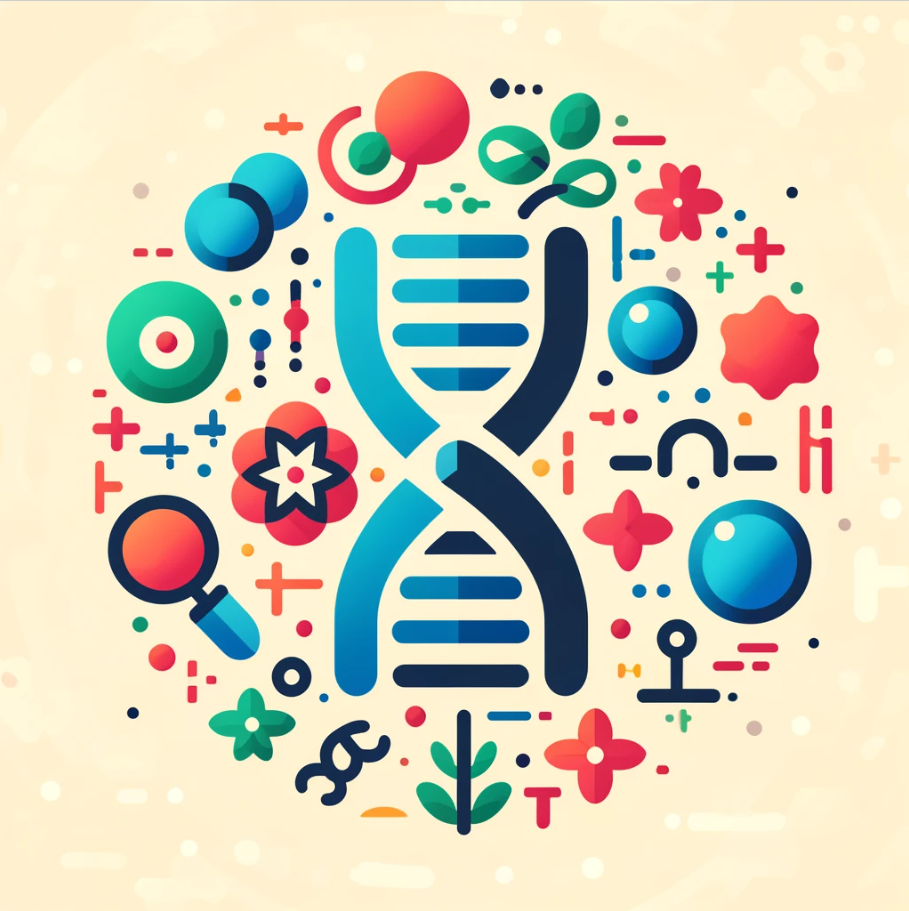
\includegraphics[width=0.5\textwidth]{./Image/IconGA.png}
		\caption{Genetic Algorithms}
		\label{fig:mylabel}
	\end{figure}
	\begin{itemize}
		\item \textbf{Thuật toán Di truyền(GA):} được phát minh bởi John Holland vào những năm 1960 tại Đại học Michigan. Mục tiêu ban đầu của Holland là tạo ra một mô hình máy tính mô phỏng các nguyên tắc của tiến hóa sinh học để nghiên cứu các quá trình thích nghi. Sau này, các nhà khoa học và các nhà nghiên cứu đã tối ưu và cải tiến thuật toán cho các bài toán khó khăn khác.
		\item \textbf{Nguyên lý cơ bản của Thuật toán Di truyền:} GA mô phỏng quá trình tiến hóa tự nhiên thông qua chọn lọc tự nhiên, lai ghép, và đột biến. GA tạo ra các thế hệ cá thể mới để tìm kiếm các giải pháp tối ưu cho một bài toán cụ thể. Vai trò của di truyền trong việc chuyển giao các đặc tính giữa các thế hệ và vai trò của đột biến trong việc duy trì sự đa dạng di truyền, từ đó giúp thuật toán khám phá ra những giải pháp mới và hiệu quả hơn.
		\item \textbf{Các bài toán sử dụng GA:} 
		\begin{itemize}
			\item Bài toán tìm mật khẩu (Find Password)
			\item Bài toán Người bán hàng (Traveling Salesman Problem - TSP)
			\item Lập lịch (Scheduling Problems)
			\item Tối ưu hóa danh mục đầu tư (Portfolio Optimization)
			\item Bài toán Đóng gói (Bin Packing Problem)
			\item Bài toán Thiết kế Mạch (Circuit Design Optimization)
			\item Tối ưu hóa Hình thức (Shape Optimization)
			\item Phân tích và Dự báo Thời tiết
			\item Robotics và Điều khiển tự động
			\item Nhận dạng Mẫu và Trí tuệ Nhân tạo
		\end{itemize}
	\end{itemize}
	\begin{figure}[h]
		\centering
		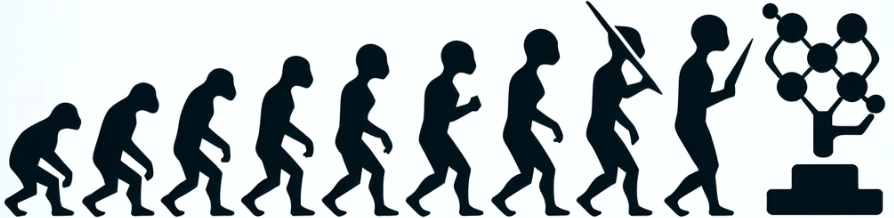
\includegraphics[width=\textwidth]{./Image/IconGACover.png}
		\label{fig:mylabel}
	\end{figure}

	\subsubsection{Các thành phần chính của GA}
	\begin{enumerate}
		\item \textbf{Mã hóa (Encoding)}
		\begin{itemize}
			\item \textit{Mục đích:} Giải thích tầm quan trọng của việc mã hóa đối với hiệu quả của GA. Mã hóa là quá trình biểu diễn các biến quyết định của bài toán thành một chuỗi, thường được gọi là chromosome.
			\item \textit{Các loại mã hóa:} Phổ biến nhất là mã hóa nhị phân, nhưng còn có mã hóa số nguyên, số thực, và mã hóa dựa trên đối tượng cho các bài toán phức tạp hơn. Mô tả ưu và nhược điểm của mỗi phương pháp.
		\end{itemize}
		\item \textbf{Khởi tạo quần thể (Population Initialization)}
		\begin{itemize}
			\item \textit{Mô tả quá trình:} Quần thể ban đầu của GA thường được sinh ra một cách ngẫu nhiên để đảm bảo sự đa dạng. Quần thể gồm nhiều cá thể, mỗi cá thể đại diện cho một giải pháp tiềm năng.
			\item \textit{Tầm quan trọng:} Khởi tạo quần thể là bước đầu tiên và quan trọng để khám phá không gian giải pháp. Số lượng cá thể trong quần thể có ảnh hưởng đến khả năng tìm kiếm và hiệu suất của GA.
		\end{itemize}
		\item \textbf{Hàm thích nghi (Fitness Function)}
		\begin{itemize}
			\item \textit{Xác định:} Hàm thích nghi là hàm đánh giá mức độ "thích hợp" của mỗi cá thể trong quần thể, thường dựa trên chất lượng của giải pháp mà cá thể đó biểu diễn.
			\item \textit{Vai trò:} Hàm thích nghi quyết định cá thể nào sẽ "sống sót" và được chọn để sinh sản trong thế hệ tiếp theo. Hàm thích nghi phải được thiết kế cẩn thận để đảm bảo rằng nó phản ánh chính xác mục tiêu của bài toán.
		\end{itemize}
		\item \textbf{Chọn lọc (Selection)}
		\begin{itemize}
			\item \textit{Mục đích:} Chọn lọc là quá trình chọn ra cá thể từ quần thể hiện tại để tạo ra cá thể cho quần thể thế hệ tiếp theo.
			\item \textit{Phương pháp:} Giới thiệu các kỹ thuật chọn lọc phổ biến như Roulette Wheel, Tournament Selection, và Stochastic Universal Sampling. Mỗi phương pháp có ưu và nhược điểm riêng trong cách thức tạo đa dạng di truyền.
		\end{itemize}
		\item \textbf{Lai ghép (Crossover)}
		\begin{itemize}
			\item \textit{Xác định:} Lai ghép là quá trình kết hợp đặc điểm của hai cá thể cha mẹ để tạo ra cá thể con.
			\item \textit{Cách thực hiện:} Mô tả các kiểu lai ghép như One-point Crossover, Two-point Crossover, và Uniform Crossover, cùng với ảnh hưởng của chúng đến đặc điểm di truyền của quần thể.
		\end{itemize}
		\item \textbf{Đột biến (Mutation)}
		\begin{itemize}
			\item \textit{Vai trò:} Đột biến giúp duy trì sự đa dạng di truyền trong quần thể bằng cách thay đổi ngẫu nhiên gen của cá thể.
			\item \textit{Phương pháp:} Giới thiệu cách thức và tỷ lệ đột biến thường được sử dụng, bao gồm Bit-flip Mutation cho mã hóa nhị phân và các phương pháp khác cho số nguyên hoặc số thực.
		\end{itemize}
	\end{enumerate}

	\begin{figure}[htbp]
		\centering
		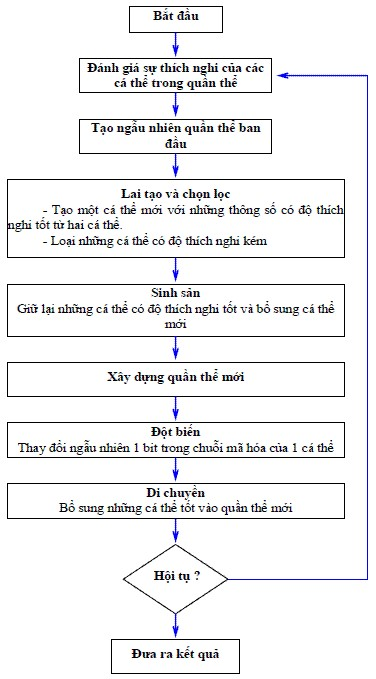
\includegraphics[width=0.5\textwidth]{./Image/So_Do_Khoi_GA.jpg}
		\caption{Sơ đồ khối GA}
		\label{fig:mylabel}
	\end{figure}
		
	\begin{figure}[htbp]
		\centering
		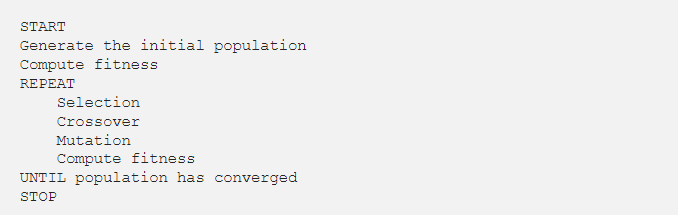
\includegraphics[width=\textwidth]{./Image/Mã giả GA.png}
		\caption{Mã giả GA}
		\label{fig:mylabel}
	\end{figure}
	\newpage
	\subsubsection{Tiêu chí đánh giá của GA}
	\begin{itemize}
		\item \textbf{Tính chính xác (Accuracy):} GA là thuật toán tìm kiếm xác suất, không đảm bảo tìm thấy giải pháp tối ưu toàn cục nhưng có khả năng tìm giải pháp tối ưu cục bộ hoặc gần với tối ưu toàn cục. Độ chính xác phụ thuộc vào hàm thích nghi, thiết kế nhiễm sắc thể, và các toán tử di truyền.
		\item \textbf{Tính khách quan (Objectivity):} GA hoạt động dựa trên chọn lọc tự nhiên, không bị ảnh hưởng bởi sự thiên vị cá nhân hay yếu tố ngoại cảnh, đảm bảo tính công bằng trong quá trình tuyển chọn.
		\item \textbf{Tính phổ dụng (Generality):} GA là phương pháp linh hoạt, áp dụng được cho nhiều loại bài toán tối ưu hóa khác nhau, từ tối ưu hóa số đến lập lịch, làm cho GA được ưa chuộng trong nhiều ngành.
		\item \textbf{Tính rõ ràng (Clarity):} Quy trình của GA rất rõ ràng và có hệ thống, bao gồm các bước khởi tạo quần thể, đánh giá hàm thích nghi, lai ghép, đột biến, và chọn lọc.
		\item \textbf{Tính kết thúc (Termination):} GA sử dụng tiêu chí kết thúc quá trình tìm kiếm như đạt số thế hệ tối đa, không cải thiện hàm thích nghi, hoặc đạt ngưỡng giá trị hàm thích nghi nhất định.
	\end{itemize}
	
	\subsubsection{Độ phức tạp}
	Độ phức tạp về thời gian của GA thường được xem xét qua ba yếu tố chính: kích thước quần thể (N), số lượng thế hệ (G), và độ phức tạp của hàm đánh giá (f). Độ phức tạp tổng thể thường được biểu diễn qua công thức:
	\begin{center}
	 \(O(N \times G \times f)\)
	\end{center}

	\begin{flushleft}
	Trong đó:
	\end{flushleft}
	 
	\begin{itemize}
		\item \(N\) là số lượng cá thể trong quần thể.
		\item \(G\) là số thế hệ.
		\item \(f\) là độ phức tạp của hàm thích nghi, có thể là \(O(1)\), \(O(n)\), \(O(n^2)\), v.v.
	\end{itemize}
	Độ phức tạp về không gian phụ thuộc vào kích thước quần thể và biểu diễn của nhiễm sắc thể, thường biểu thị qua \(O(N \times s)\), với \(s\) là không gian lưu trữ cần thiết cho mỗi cá thể.
	\subsubsection{Bài toán điển hình}
	\textbf{Bài toán Đoán Mật Khẩu (Password Guessing Problem):} Trong bài toán này, mục tiêu là tìm ra một chuỗi ký tự bằng cách 'đoán' liên tục. GA sử dụng các toán tử di truyền như lai ghép và đột biến để tạo ra các thế hệ mới của các chuỗi ký tự, tiến tới mật khẩu đúng. Đây là minh họa hiệu quả của cách mà GA tối ưu hóa và tiến hóa dần tới giải pháp qua nhiều thế hệ.
	
	\begin{flushleft}
		\textbf{Ví dụ minh họa: }
		Xét bài toán Tìm mật khẩu với các yêu cầu sau:
		\begin{itemize}
			\item Mật khẩu gồm 8 kí tự, bao gồm chữ cái, chữ số và khoảng trắng. Ví dụ mật khẩu: \texttt{hoilamgi}.
			\item Mỗi lần thử, hệ thống sẽ báo về số lượng kí tự đúng với mật khẩu.
			\item Yêu cầu tìm ra chuỗi mật khẩu đã cho trước.
		\end{itemize}
	\end{flushleft}

	\begin{center}
		
		
		
		\begin{figure}[htbp]
			\centering
			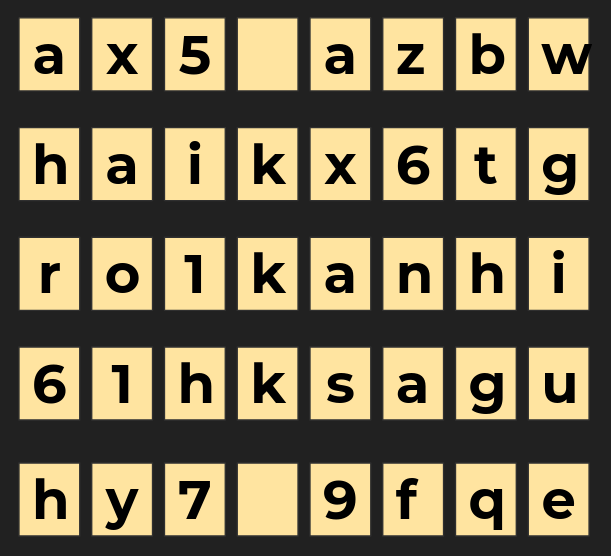
\includegraphics[width=0.6\textwidth]{./Image/step1.png}
			\caption{Khởi tạo quần thể bất kỳ với chiều dài mỗi mật khẩu là 8 ký tự }
			\label{fig:mylabel}
		\end{figure}
		\begin{figure}[htbp]
			\centering
			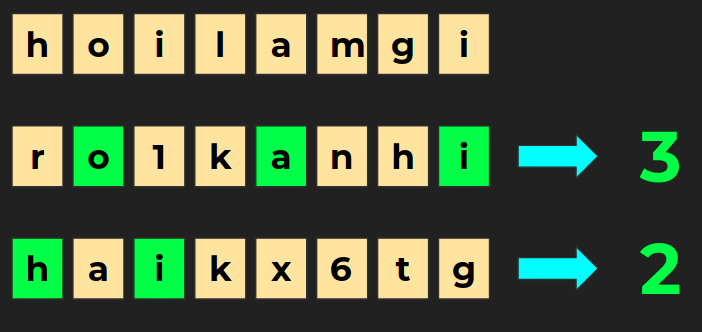
\includegraphics[width=0.7\textwidth]{./Image/step2.png}
			\caption{Đánh giá mật khẩu trong quần thể }
			\label{fig:mylabel}
		\end{figure}
		\begin{figure}[htbp]
			\centering
			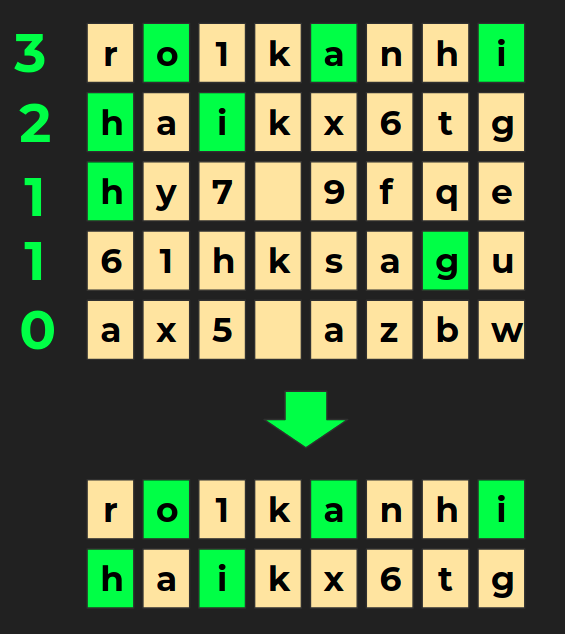
\includegraphics[width=0.6\textwidth]{./Image/step3.png}
			\caption{lựa chọn cặp bố mẹ khỏe nhất sau khi đánh giá}
			\label{fig:mylabel}
		\end{figure}
		\begin{figure}[htbp]
			\centering
			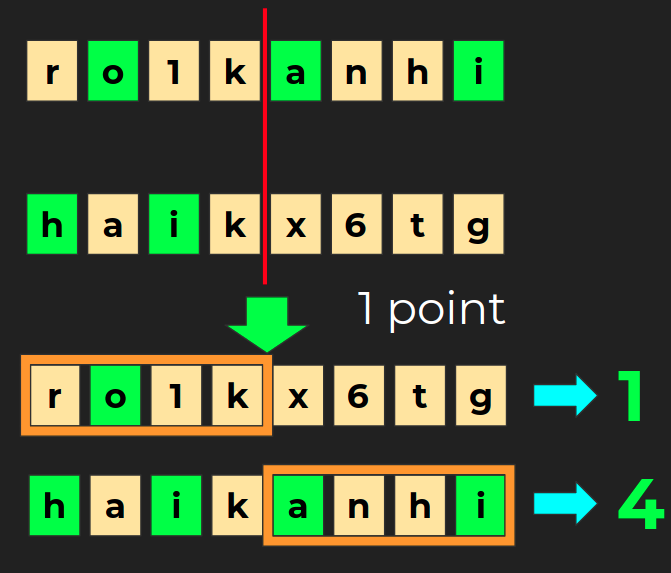
\includegraphics[width=0.3\textwidth]{./Image/step4.png}
			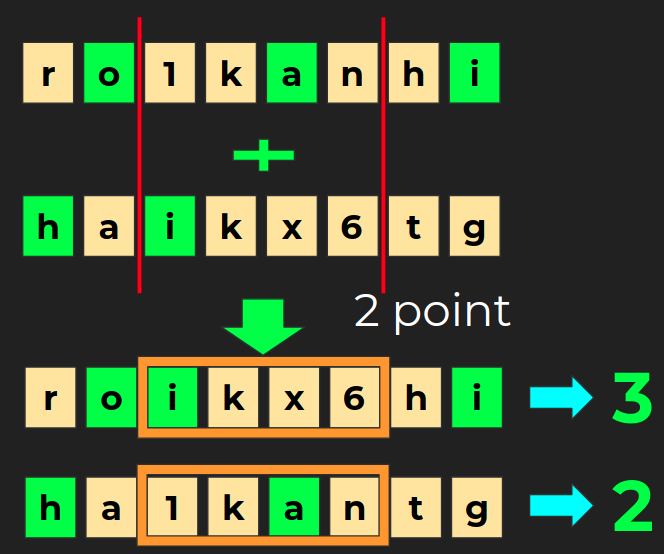
\includegraphics[width=0.305\textwidth]{./Image/step5.png}
			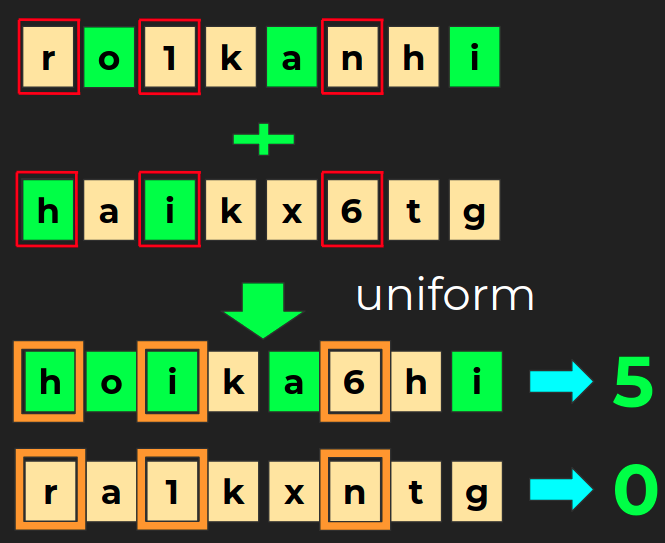
\includegraphics[width=0.31\textwidth]{./Image/step6.png}
			\caption{a,b,c: Lai ghép cặp bố mẹ rồi đánh giá cặp con tương ứng}
			\label{fig:mylabel}
		\end{figure}
		\begin{figure}[htbp]
			\centering
			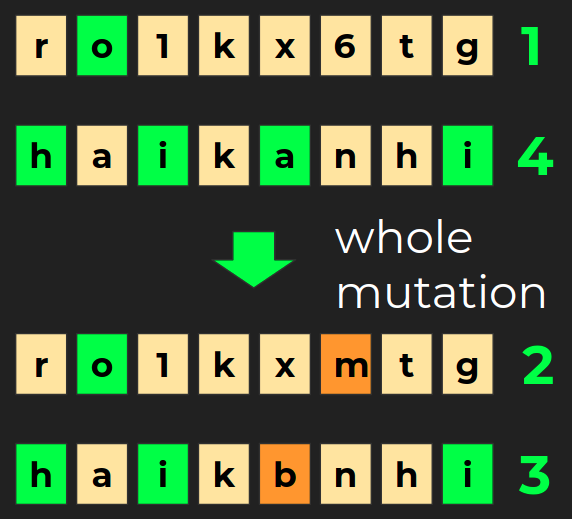
\includegraphics[width=0.6\textwidth]{./Image/step7.png}
			\caption{Đột biến con lai tạo sau khi lai ghép}
			\label{fig:mylabel}
		\end{figure}
	\end{center}
	\newpage
	\subsubsection{Các biến thể của GA}
	\newpage
	\begin{enumerate}
		\item \textbf{Steady-State Genetic Algorithm (SSGA):}
		\begin{itemize}
			\item Đặc điểm: Trong SSGA, một hoặc một số cá thể mới được tạo ra và ngay lập tức thay thế một số cá thể kém thích nghi nhất trong quần thể, thay vì thay thế toàn bộ quần thể như trong GA tiêu chuẩn.
			\item Ưu điểm: Giúp duy trì sự ổn định của quần thể và thường nhanh chóng hội tụ hơn so với GA tiêu chuẩn.
		\end{itemize}
		\begin{figure}[htbp]
			\centering
			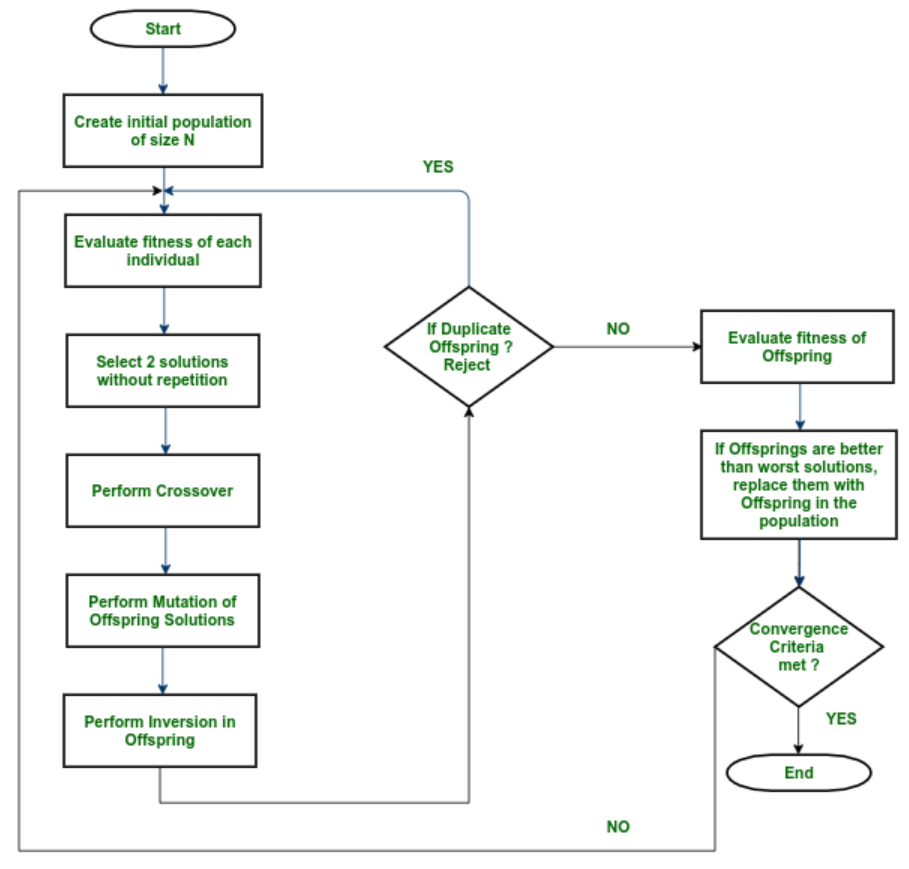
\includegraphics[width=0.7\textwidth]{./Image/sơ đồ khối SSGA.png}
			\caption{Sơ đồ khối SSGA}
			\label{fig:mylabel}
		\end{figure}
		\newpage
		\item \textbf{Elitist Genetic Algorithm:}
		\begin{itemize}
			\item Đặc điểm: Phương pháp này bảo tồn một hoặc một số cá thể tốt nhất trong mỗi thế hệ (elites) không bị thay thế trong quá trình sinh sản.
			\item Ưu điểm: Ngăn chặn mất mát của các giải pháp tốt nhất đã tìm thấy, đảm bảo rằng hiệu suất của quần thể không giảm qua các thế hệ.
		\end{itemize}
	
		\begin{figure}[htbp]
			\centering
			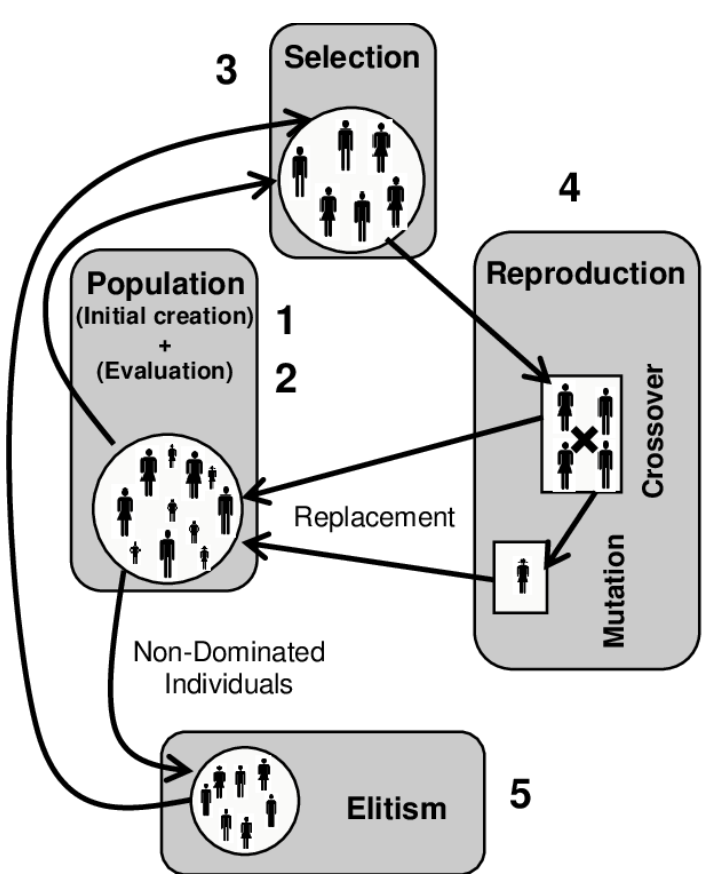
\includegraphics[width=0.7\textwidth]{./Image/Sơ đồ khối Elitist Genetic Algorithm.png}
			\caption{Sơ đồ khối Elitist Genetic Algorithm}
			\label{fig:mylabel}
		\end{figure}
		\newpage
		\item \textbf{Multi-Objective Genetic Algorithms (MOGA):}
		\begin{itemize}
			\item Đặc điểm: Được thiết kế để giải quyết các bài toán có nhiều mục tiêu tối ưu hóa đồng thời, mà không cần chuyển đổi chúng thành một mục tiêu đơn lẻ.
			\item Ưu điểm: Có khả năng tìm ra một tập hợp các giải pháp tối ưu đa dạng, mỗi giải pháp tốt ở một mục tiêu nhất định, gọi là Pareto front.
		\end{itemize}
		\begin{figure}[htbp]
			\centering
			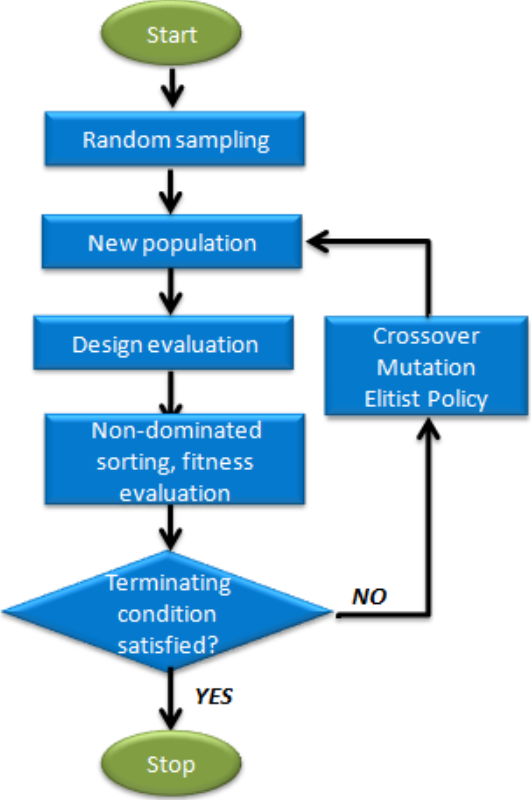
\includegraphics[width=0.5\textwidth]{./Image/Sơ đồ khối Multi-Objective Genetic Algorithms.png}
			\caption{Sơ đồ khối Multi-Objective Genetic Algorithms (MOGA)}
			\label{fig:mylabel}
		\end{figure}
	
		\newpage
		\item \textbf{Adaptive Genetic Algorithms:}
		\begin{itemize}
			\item Đặc điểm: Tự động điều chỉnh các tham số của GA (như tỷ lệ đột biến, tỷ lệ lai ghép) dựa trên tiến trình tối ưu hóa.
			\item Ưu điểm: Tăng khả năng thích ứng với bài toán cụ thể, cải thiện hiệu quả tìm kiếm và hội tụ.
		\end{itemize}
		\begin{figure}[htbp]
			\centering
			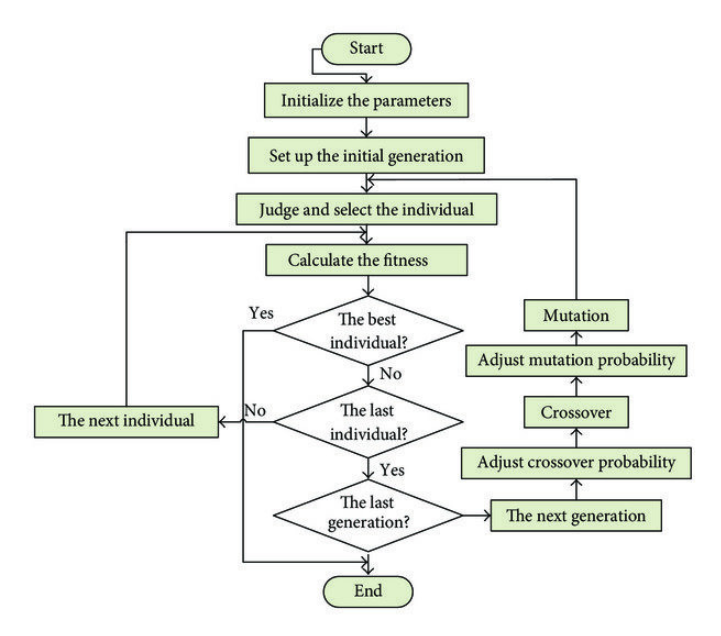
\includegraphics[width=\textwidth]{./Image/Sơ đồ khối Adaptive Genetic Algorithms.png}
			\caption{Sơ đồ khối Adaptive Genetic Algorithms}
			\label{fig:mylabel}
		\end{figure}
	
		\newpage
		\item \textbf{Hybrid Genetic Algorithms:}
		\begin{itemize}
			\item Đặc điểm: Kết hợp GA với các kỹ thuật tối ưu hóa khác (như Hill Climbing, Simulated Annealing, hoặc thậm chí là các thuật toán khác như Particle Swarm Optimization).
			\item Ưu điểm: Tận dụng điểm mạnh của từng phương pháp để cải thiện hiệu quả tìm kiếm và khả năng hội tụ, đặc biệt hữu ích cho các bài toán phức tạp.
		\end{itemize}
	
		\begin{figure}[htbp]
			\centering
			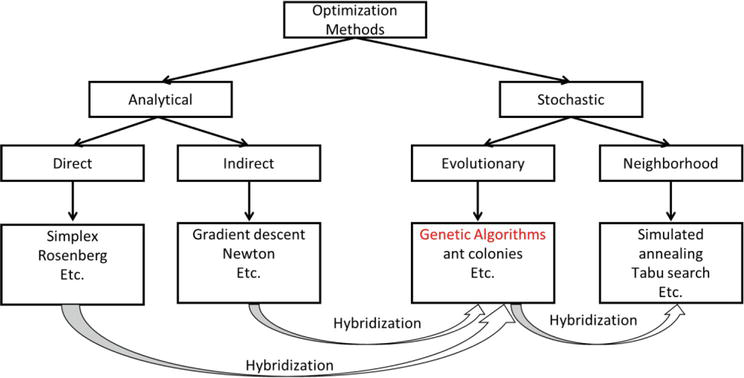
\includegraphics[width=0.7\textwidth]{./Image/Sơ đồ khối Hybrid Genetic Algorithms.png}
			\caption{Sơ đồ khối Hybrid Genetic Algorithms}
			\label{fig:mylabel}
		\end{figure}
	
		\item \textbf{Parallel Genetic Algorithms:}
		\begin{itemize}
			\item Đặc điểm: Phân tán quá trình GA trên nhiều máy tính hoặc nhiều luồng xử lý để thực hiện đồng thời.
			\item Ưu điểm: Giảm thời gian tính toán đáng kể, đặc biệt quan trọng cho các bài toán lớn.
		\end{itemize}
	
		\begin{figure}[htbp]
			\centering
			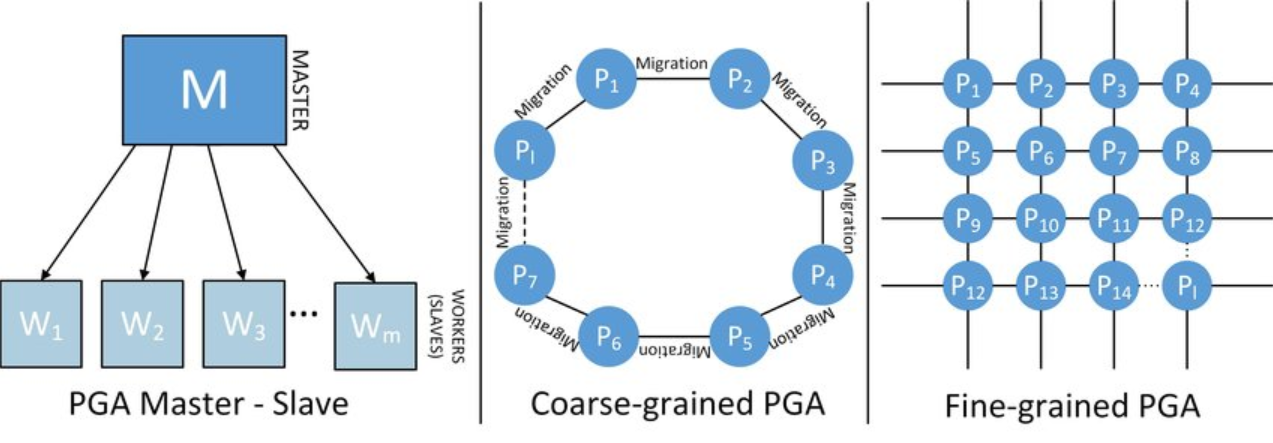
\includegraphics[width=0.7\textwidth]{./Image/Sơ đồ khối Parallel Genetic Algorithms.png}
			\caption{Sơ đồ khối Parallel Genetic Algorithms}
			\label{fig:mylabel}
		\end{figure}
	
		\newpage
		\item \textbf{Real-Coded Genetic Algorithms:}
		\begin{itemize}
			\item Đặc điểm: Sử dụng biểu diễn số thực thay vì chuỗi nhị phân để mã hóa các biến số.
			\item Ưu điểm: Cải thiện độ chính xác và hiệu quả của GA trong các bài toán có biến số liên tục.
		\end{itemize}
	
		\begin{figure}[htbp]
			\centering
			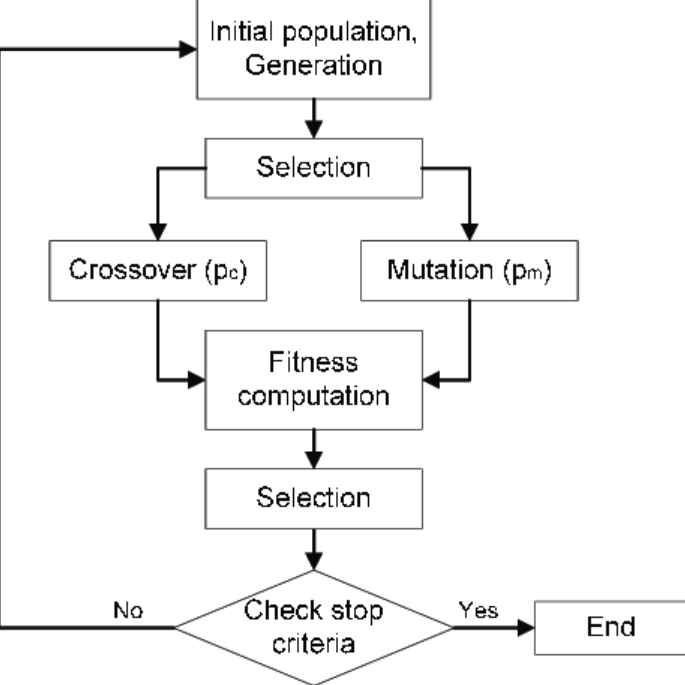
\includegraphics[width=0.7\textwidth]{./Image/Sơ đồ khối Real-Coded Genetic Algorithms.png}
			\caption{Sơ đồ khối Real-Coded Genetic Algorithms}
			\label{fig:mylabel}
		\end{figure}
	
		\newpage
		\item \textbf{Constraint-Handling Techniques in GA:}
		\begin{itemize}
			\item Đặc điểm: Áp dụng các kỹ thuật đặc biệt để xử lý các ràng buộc trong bài toán, giúp GA có thể áp dụng cho các bài toán tối ưu hóa có ràng buộc.
			\item Ưu điểm: Mở rộng khả năng áp dụng của GA cho một loạt các bài toán thực tế có các ràng buộc phức tạp.
		\end{itemize}
	
		\begin{figure}[htbp]
			\centering
			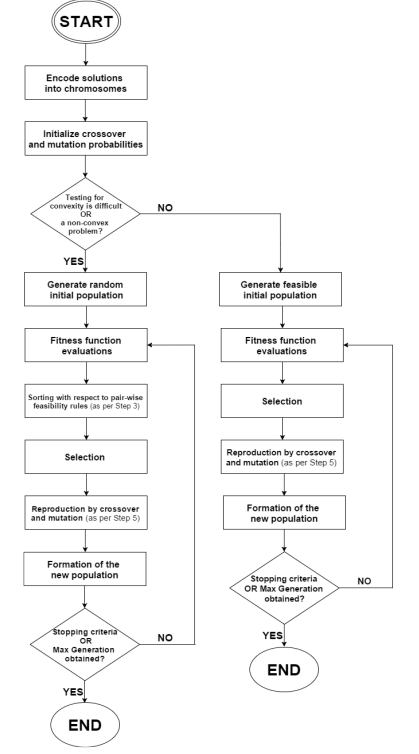
\includegraphics[width=0.5\textwidth]{./Image/Sơ đồ khối Constraint-Handling Techniques in GA.png}
			\caption{Sơ đồ khối Constraint-Handling Techniques in GA}
			\label{fig:mylabel}
		\end{figure}
	
	\end{enumerate}
	\newpage
	\subsection{Thuật toán tối ưu hóa đàn kiến (ACO)}
	\begin{figure}[htbp]
		\centering
		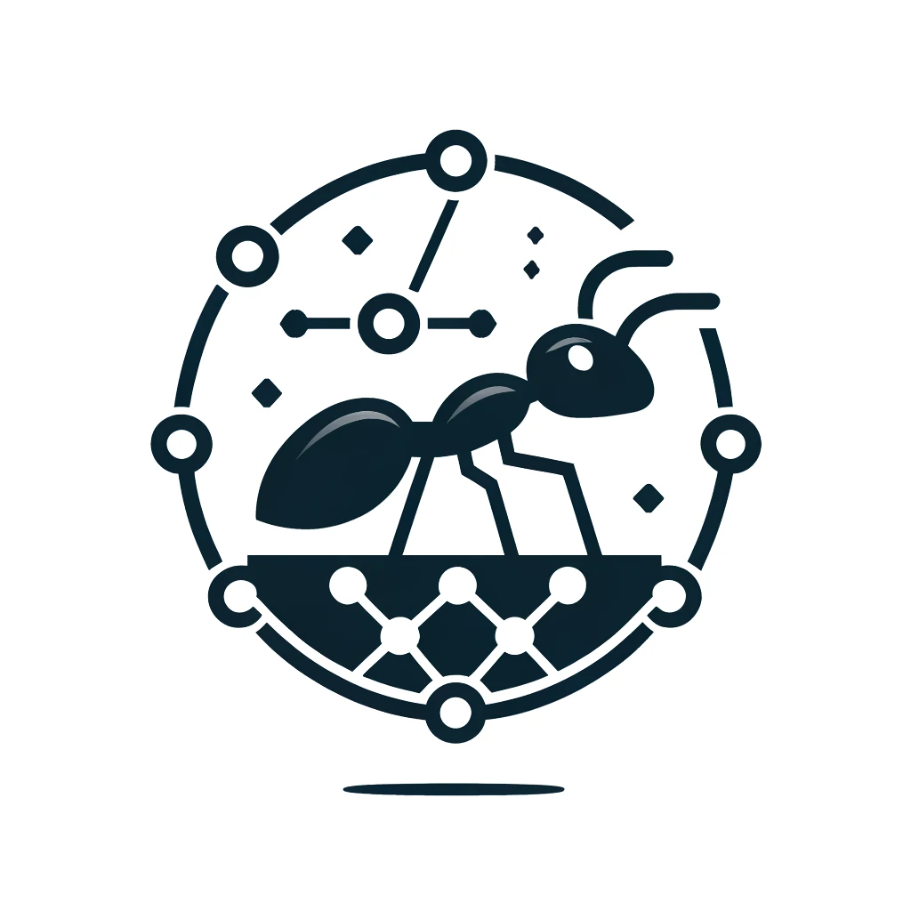
\includegraphics[width=0.4\textwidth]{./Image/IconACO.png}
		\label{fig:mylabel}
	\end{figure}
	\begin{itemize}
		\item \textbf{Thuật toán tối ưu hóa đàn kiến (ACO):} được phát triển bởi Marco Dorigo vào đầu những năm 1990 trong khuôn khổ luận án tiến sĩ của ông tại Đại học Libre de Bruxelles, Bỉ. Thuật toán ban đầu được thiết kế để giải quyết bài toán người bán hàng (Travelling Salesman Problem - TSP), một trong những bài toán tối ưu hóa tổ hợp phổ biến và thách thức.
		\item \textbf{Nguyên lý cơ bản của Thuật toán tối ưu hóa đàn kiến:} lấy cảm hứng từ hành vi tìm đường và xây dựng tổ của loài kiến trong tự nhiên. Khi kiếm ăn, kiến phát tán một chất hóa học gọi là pheromone trên đường đi của chúng. Các con kiến khác có thể cảm nhận được mùi pheromone và theo dõi nó để tìm thức ăn. Đường đi có nhiều pheromone hơn (tức là được nhiều kiến đi qua) trở nên hấp dẫn hơn, dẫn đến một quá trình tối ưu hóa tự nhiên qua đó đường đi tốt nhất dần được thiết lập
		\item \textbf{Các bài toán sử dụng ACO:} 
		\begin{itemize}
			\item Bài toán Người bán hàng (Traveling Salesman Problem - TSP)
			\item Bài toán lập lịch (Scheduling Problems)
			\item Bài toán Vận tải (Vehicle Routing Problem - VRP)
			\item Bài toán cắt ghép (Cutting Stock Problem)
			\item Tối ưu hóa định tuyến mạng (Network Routing Optimization)
			\item Tối ưu hóa danh mục đầu tư (Portfolio Optimization)
			\item Bài toán gán công việc (Assignment Problems)
			\item Bài toán tổ hợp (Combinatorial Optimization)
			\item V.v...
		\end{itemize}
	\end{itemize}
	\begin{figure}[htbp]
		\centering
		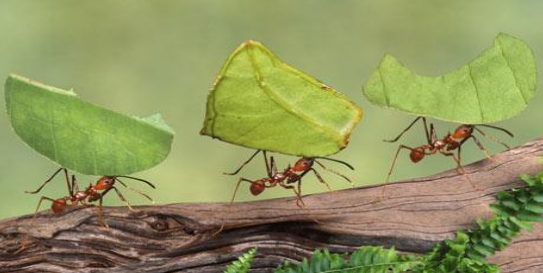
\includegraphics[width=\textwidth]{./Image/IconACO_Cover.png}
		\label{fig:mylabel}
	\end{figure}
	\newpage
	\subsubsection{Các thành phần chính của ACO}
	
	\begin{enumerate}
	\item \textbf{Kiến (Ants):}
	\begin{itemize}
		\item \textit{Mô tả:} Trong ACO, kiến được mô phỏng là các tác nhân giải quyết bài toán. Chúng bắt đầu từ một điểm, thường là điểm khởi đầu của bài toán, và dần dần xây dựng lộ trình bằng cách lựa chọn từng bước tiếp theo dựa trên pheromone và thông tin heuristic.
		\item \textit{Vai trò:} Tác nhân của thuật toán, mỗi con kiến tương ứng với một lần chạy thuật toán hoặc một lần thử nghiệm giải pháp, và chúng cộng tác để khám phá không gian giải pháp.
	\end{itemize}
	
	\item \textbf{Pheromone:}
	\begin{itemize}
		\item \textit{Mô tả:} Pheromone trong ACO là một biến số ảo mà kiến "để lại" trên lộ trình mà chúng đã đi qua. Lượng pheromone trên một lộ trình phản ánh mức độ thành công của lộ trình đó trong quá khứ, càng nhiều kiến đi qua và càng thành công thì lượng pheromone càng cao.
		\item \textit{Vai trò:} Đây là cơ chế chính để chia sẻ thông tin giữa các kiến, giúp thuật toán tập trung vào những lộ trình tốt hơn và tránh những lộ trình kém hiệu quả.
	\end{itemize}
	
	\item \textbf{Heuristic Information:}
	\begin{itemize}
		\item \textit{Mô tả:} Thông tin heuristic là dữ liệu dựa trên bản chất của bài toán, chẳng hạn như khoảng cách giữa các điểm trong bài toán người bán hàng, hoặc chi phí liên quan đến một bước chuyển động trong bài toán tối ưu hóa.
		\item \textit{Vai trò:} Hỗ trợ kiến trong việc lựa chọn bước tiếp theo bằng cách cung cấp một "mức độ ưu tiên" tự nhiên dựa trên các tính toán đơn giản, giúp kết hợp sự khám phá ngẫu nhiên với việc tập trung vào giải pháp hiệu quả.
	\end{itemize}
	
	\item \textbf{Hàm Mục tiêu (Objective Function):}
	\begin{itemize}
		\item \textit{Mô tả:} Hàm mục tiêu là tiêu chuẩn để đánh giá chất lượng của một lộ trình hoặc giải pháp. Trong ACO, hàm mục tiêu thường được dùng để tính toán "mức độ thích hợp" của một lộ trình dựa trên tổng chi phí, khoảng cách, thời gian, hoặc các yếu tố tương tự.
		\item \textit{Vai trò:} Xác định mức độ cập nhật pheromone trên các lộ trình; lộ trình càng tối ưu theo hàm mục tiêu, lượng pheromone để lại càng nhiều, từ đó hướng dẫn các kiến trong các lần tìm kiếm sau tập trung vào những lộ trình đó.
	\end{itemize}
	\end{enumerate}
		\begin{figure}[htbp]
		\centering
		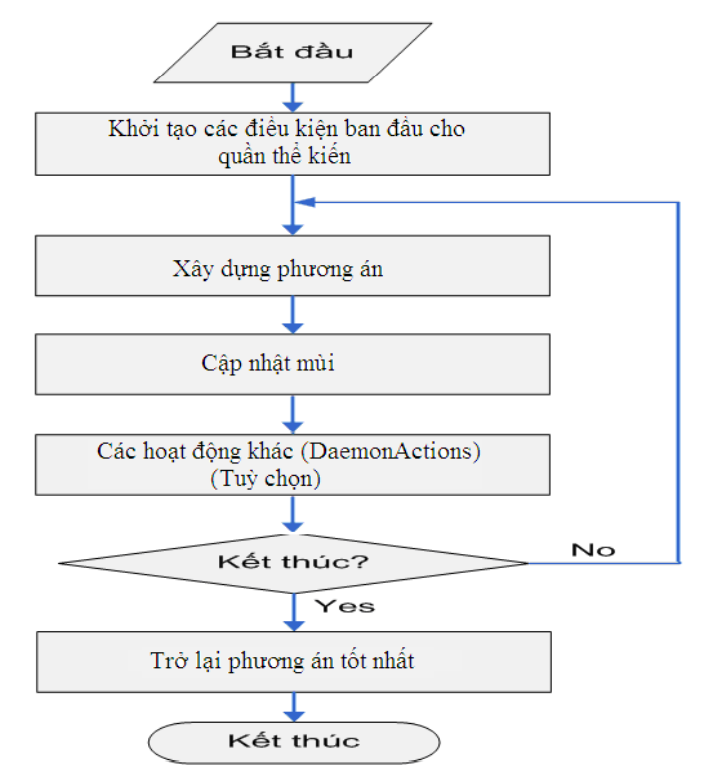
\includegraphics[width=0.5\textwidth]{./Image/Sơ đồ khối ACO.png}
		\caption{Sơ đồ khối ACO}
		\label{fig:mylabel}
	\end{figure}

	\begin{figure}[htbp]
		\centering
		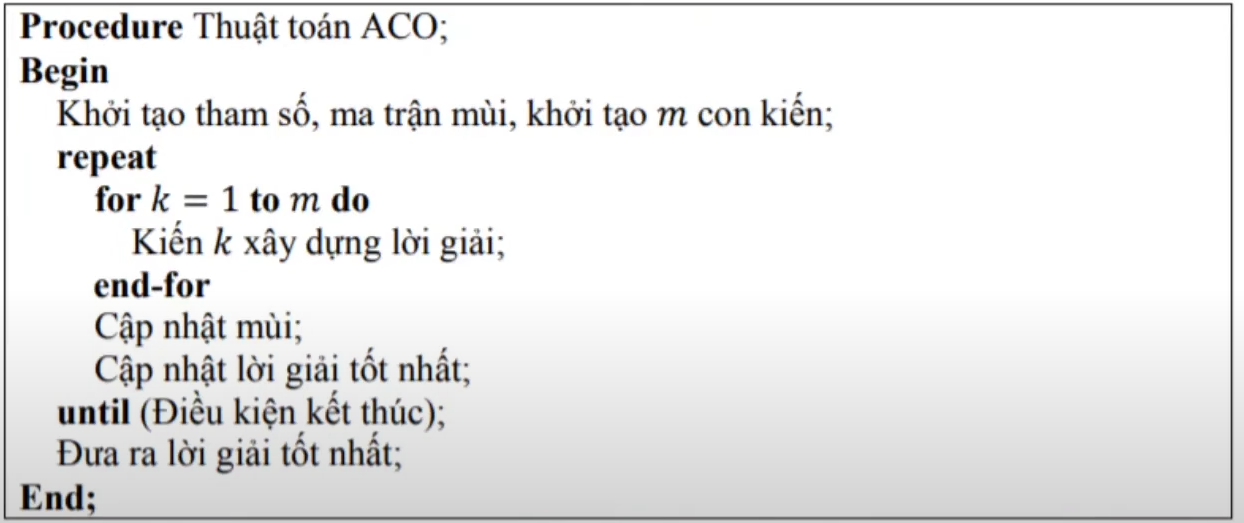
\includegraphics[width=\textwidth]{./Image/Mã giả ACO.png}
		\caption{Mã giả ACO}
		\label{fig:mylabel}
	\end{figure}	
	\newpage
	\subsubsection{Tiêu chí đánh giá của ACO}
	
	\begin{itemize}
		\item \textbf{Tính chính xác (Accuracy):} ACO đạt được tính chính xác thông qua việc cập nhật đường đi tốt nhất dựa trên lượng pheromone mà các "kiến" để lại trên đường đi của chúng. Khi nhiều kiến lựa chọn một đường đi và để lại pheromone, đường đi đó trở nên hấp dẫn hơn, dẫn đến khả năng cao mà đường đó là lối đi tối ưu hoặc gần tối ưu. Tuy nhiên, ACO không đảm bảo tìm được giải pháp tối ưu toàn cục 100% trong mọi trường hợp, nhưng nó thường tìm được giải pháp rất tốt trong thực tế.
		\item \textbf{Tính khách quan (Objectivity):} ACO hoạt động dựa trên quy tắc khách quan là mức độ tích lũy pheromone, không phụ thuộc vào bất kỳ yếu tố chủ quan nào khác từ bên ngoài. Tuy nhiên, cách thiết lập tham số ban đầu và cập nhật pheromone có thể ảnh hưởng đến kết quả, nhưng nhìn chung, quá trình tìm kiếm giải pháp của ACO là khách quan vì nó dựa trên thông tin mà kiến thu thập được.
		\item \textbf{Tính phổ dụng (Generality):} ACO được áp dụng rộng rãi cho nhiều loại bài toán tối ưu hóa, từ bài toán người du lịch (TSP) đến các bài toán lập lịch và phân bổ tài nguyên. Sự linh hoạt này là do cơ chế tự thích ứng của ACO, cho phép nó tìm kiếm giải pháp hiệu quả trong nhiều không gian tìm kiếm khác nhau.
		\item \textbf{Tính rõ ràng (Clarity):} Mặc dù ACO là một thuật toán phức tạp, các bước của nó khá rõ ràng: khởi tạo pheromone, kiến di chuyển dựa trên pheromone và hàm giá trị, cập nhật pheromone dựa trên chất lượng của lối đi, và lặp lại quá trình. Cách tiếp cận này là minh bạch và có thể được theo dõi dễ dàng trong các bước triển khai.
		\item \textbf{Tính kết thúc (Termination):} ACO thường sử dụng một số tiêu chí dừng cụ thể, như số lần lặp tối đa, không có cải thiện trong chất lượng đường đi sau nhiều lần lặp, hoặc đạt được một giải pháp có độ chính xác nhất định. Điều này giúp đảm bảo rằng thuật toán không chạy vô hạn và tài nguyên tính toán được sử dụng một cách hiệu quả.
	\end{itemize}
	
	\subsubsection{Độ phức tạp}
	Độ phức tạp của Thuật toán Tối ưu Hóa Bầy Kiến (Ant Colony Optimization - ACO) có thể khá phức tạp để phân tích chính xác vì nó phụ thuộc vào nhiều yếu tố như kích thước của bài toán, số lượng kiến trong mô phỏng, và cách thức cập nhật pheromone.
	\begin{enumerate}
		\item\textbf{Độ phức tạp thời gian:}
		\begin{enumerate}
			\item\textbf{Số lượng kiến (m):} Mỗi con kiến trong quần thể tạo một lộ trình hoàn chỉnh trong bài toán.
			
			\item\textbf{Số thành phần (n):} Đây có thể là số lượng thành phố trong TSP. Mỗi kiến cần xem xét mỗi thành phần để xây dựng lộ trình.
			
			\item\textbf{Số lần lặp (t):}  Đại diện cho số lần thuật toán thực hiện quá trình tìm kiếm giải pháp, bao gồm cả việc cập nhật pheromone.
			
			\item\textbf{Chi phí tính toán cho mỗi lượt di chuyển của kiến (c):} Đây là chi phí để mỗi con kiến tạo ra một lộ trình hoàn chỉnh. Trong trường hợp tồi tệ nhất, chi phí này có thể là \(O(n^{2})\), khi mỗi con kiến xem xét mọi cặp thành phần có thể.

			 \item\textbf{Độ phức tạp thời gian tổng thể của ACO có thể là:} 
			\begin{center}
				\(O(t \times m \times c)\)
			\end{center}
			
			
			\item Trong đó t là số lần lặp, m là số lượng kiến, và  đại diện cho chi phí tạo một lộ trình hoàn chỉnh của một kiến, giả sử mỗi kiến cần xem xét mọi cặp thành phần có thể. Đây là ước lượng cho trường hợp phức tạp nhất, trong thực tế, tùy vào thiết kế cụ thể của thuật toán và các cải tiến được áp dụng, độ phức tạp có thể thấp hơn.
		\end{enumerate}
	
		\item\textbf{Độ phức tạp không gian}
		\begin{enumerate}
			\item ACO cũng yêu cầu một lượng lớn bộ nhớ để lưu trữ thông tin pheromone trên mọi cạnh của đồ thị, điều này có độ phức tạp không gian là: \(O(n^{2})\)
			
			\item Đối với bài toán như TSP, nơi pheromone cần được lưu trữ cho mỗi cặp thành phố.
			
		\end{enumerate}
		
	\end{enumerate}
	\subsubsection{Bài toán điển hình}
	Bài toán tìm đường đi ngắn nhất giữa điểm bắt đầu tới điểm đích là 1 bài toán điển hình của ACO nhằm tối ưu đường đi tới đích một cách ngắn nhất nhanh nhất.
	
	\textbf{Ví dụ:} Cho 4 đình A, B, C, D với AB=BD = 1 , AC=CD=0.5 đơn vị khoảng cách tổ kiến bắt đầu từ A và thức ăn tại D. Tìm đường đi ngắn nhất
	\begin{figure}[htbp]
		\centering
		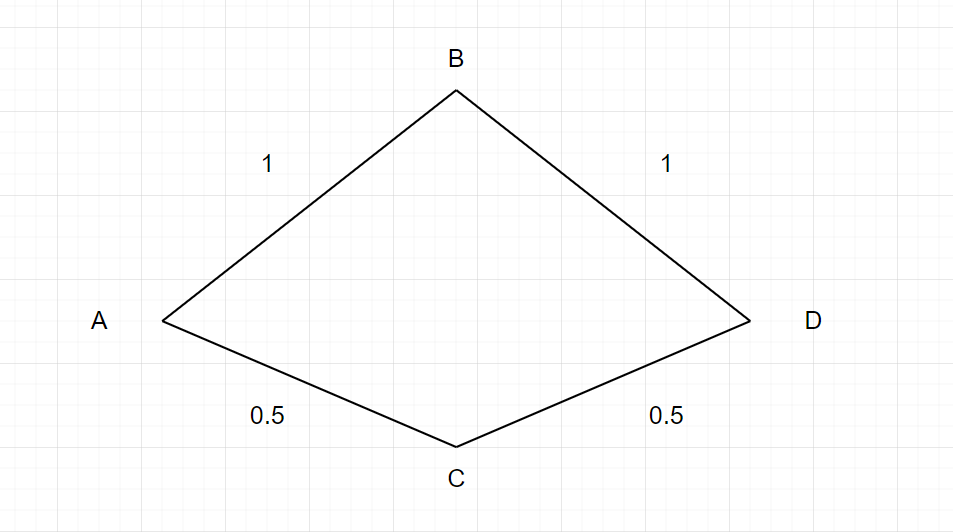
\includegraphics[width=\textwidth]{./Image/Sơ đồ đường đi ví dụ.png}
		\caption{Sơ đồ đường đi ví dụ}
		\label{fig:mylabel}
	\end{figure}
	\newpage
	\paragraph{Khởi tạo các giá trị :}
		\begin{itemize}
			\item $\tau_{A,B}, \tau_{A,C}$: Mức pheromone ban đầu trên các cạnh A-B và A-C. Giả sử ban đầu là 0.1 cho cả hai cạnh
			
			\item $\eta_{A,B}, \eta_{A,C}$: Độ thuận lợi của cạnh, tính bằng nghịch đảo của khoảng cách từ A đến B và từ A đến C. Với khoảng cách AB = 1 và AC = 0.5, ta có $\eta_{A,B} = \frac{1}{1} = 1$ và $\eta_{A,C} = \frac{1}{0.5} = 2$.
			
			
			\item $\alpha, \beta$: Các tham số điều chỉnh ảnh hưởng của pheromone ($\alpha$) và thông tin heuristic ($\beta$). Giả sử $\alpha=1$, $\beta=2$.
			
		\end{itemize}
	\paragraph{Công thức tính xác suất:}
	Xác suất P$\_{i,j}$ để kiến chọn đi từ điểm i đến j được tính bằng công thức: 
		\begin{center}
			\[
			P_{i,j} = \frac{(\tau_{i,j})^\alpha \cdot (\eta_{i,j})^\beta}{\sum_{k \in \j(i)} (\tau_{i,k})^\alpha \cdot (\eta_{i,k})^\beta}
			\]
		\end{center}
	\paragraph{Xác suất từ A đến B (P$\_{A,B}$):}
		\begin{center}
			\[
			P_{A,B} = \frac{(0.1)^1 \cdot (1)^2}{(0.1)^1 \cdot (1)^2 + (0.1)^1 \cdot (2)^2} = \frac{0.1}{0.5} = 0.2
			\]
		\end{center}
		\textbf{Giải thích:}
		\begin{enumerate}
			\item $\tau_{A,B}, \tau_{A,C}$ = 0.1
			
			\item $\eta_{A,B} = 1, \eta_{A,C} = 2$
			
			\item $\alpha = 1, \beta = 2$
		\end{enumerate}
	\paragraph{Xác suất từ A đến C (P$\_{A,C}$):}
	\begin{center}
		\[
		P_{A,C} = \frac{(0.1)^1 \cdot (2)^2}{(0.1)^1 \cdot (1)^2 + (0.1)^1 \cdot (2)^2} = \frac{0.4}{0.5} = 0.8
		\]
	\end{center}
	\paragraph{=>} Từ đó kiến sẽ chọn đường đi có xác suất cao nhất để đi. Nhưng vẫn còn có trong số các con kiến đi đường có xác suất ít để đi và kiểm tra đường đi khác, vì đâu chắc tổng đường đi chứa đường có xác suất nhỏ nhất đang xét nó nhỏ hơn tổng đường đi của các đường chứa đường có xác xuất lớn hơn.
	
	\newpage
	\subsubsection{Các biến thể của ACO}
	
	\begin{enumerate}
		\item \textbf{Ant System (AS)}
		\begin{itemize}
			\item \textit{Mô tả:} AS là phiên bản ban đầu của ACO. Trong AS, tất cả kiến được cho là cập nhật pheromone dựa trên chất lượng của lộ trình mà chúng đã tìm thấy.
			\item \textit{Ứng dụng:} Phù hợp cho các bài toán có không gian tìm kiếm không quá lớn, nơi mà sự thăm dò có thể được thực hiện một cách có hệ thống.
		\end{itemize}
		
		\item \textbf{Ant Colony System (ACS)}
		\begin{itemize}
			\item \textit{Mô tả:} Trong ACS, chỉ những kiến tìm thấy lộ trình tốt nhất mới được cập nhật pheromone, điều này giúp tập trung vào việc khai thác các lộ trình tối ưu.
			\item \textit{Ứng dụng:} Đặc biệt hiệu quả trong các bài toán đòi hỏi khả năng khai thác nhanh chóng các giải pháp tốt.
		\end{itemize}
		
		\item \textbf{Max-Min Ant System (MMAS)}
		\begin{itemize}
			\item \textit{Mô tả:} MMAS đặt giới hạn trên và dưới cho lượng pheromone, ngăn chặn sự thống trị của bất kỳ lộ trình nào để đảm bảo sự khám phá đầy đủ hơn của không gian tìm kiếm.
			\item \textit{Ứng dụng:} Phù hợp cho các bài toán có nguy cơ cao bị mắc kẹt ở cực tiểu địa phương.
		\end{itemize}
		\begin{figure}[htbp]
			\centering
			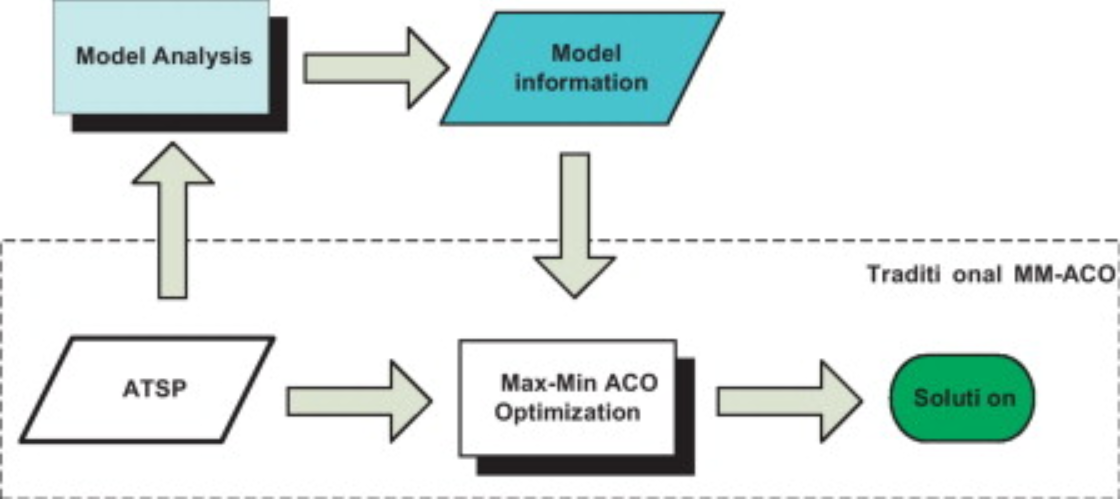
\includegraphics[width=\textwidth]{./Image/Mô hình Max-Min Ant System.png}
			\caption{Mô hình Max-Min Ant System}
			\label{fig:mylabel}
		\end{figure}
	
		\item \textbf{Ant\_Q-learning}
		\begin{itemize}
			\item \textit{Mô tả:} Là sự kết hợp giữa ACO và Q-learning, một kỹ thuật học tăng cường. Trong Ant-Q, kiến cập nhật giá trị của pheromone dựa trên một quá trình học có thưởng thức.
			\item \textit{Ứng dụng:} Hiệu quả trong các môi trường động, nơi các kiến cần thích ứng với sự thay đổi của bài toán theo thời gian.
		\end{itemize}
		\newpage
		\item \textbf{Rank-based Ant System (RAS)}
		\begin{itemize}
			\item \textit{Mô tả:} Chỉ những kiến tìm thấy các lộ trình tốt nhất mới được phép cập nhật pheromone, nhưng dựa trên xếp hạng thay vì chỉ có một kiến tốt nhất.
			\item \textit{Ứng dụng:} Cung cấp sự cân bằng tốt hơn giữa khám phá và khai thác, thích hợp cho các bài toán có không gian tìm kiếm rộng.
		\end{itemize}
		\begin{figure}[htbp]
			\centering
			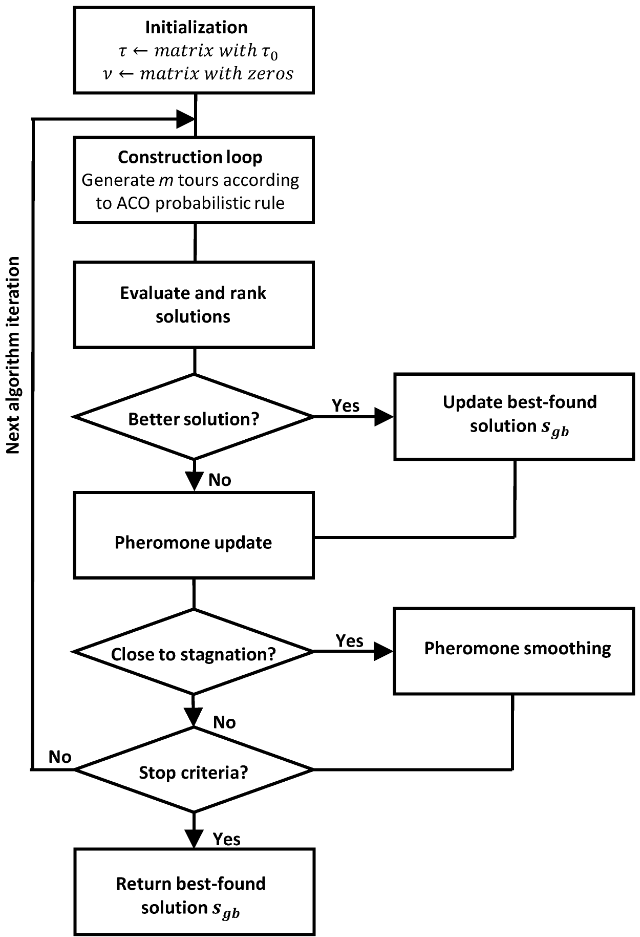
\includegraphics[width=0.5\textwidth]{./Image/Mô hình Rank-based Ant System.png}
			\caption{Mô hình Rank-based Ant System}
			\label{fig:mylabel}
		\end{figure}
	
		\item \textbf{Hypercube Framework for Ant Colony Optimization (HACO)}
		\begin{itemize}
			\item \textit{Mô tả:} Trong HACO, pheromone được xử lý trong một không gian nhiều chiều, cho phép thể hiện phức tạp hơn các mối quan hệ giữa các thành phần.
			\item \textit{Ứng dụng:} Đặc biệt hữu ích trong các bài toán tối ưu hóa đa mục tiêu hoặc khi các quyết định có mối liên hệ phức tạp với nhau.
		\end{itemize}
	\end{enumerate}
	\newpage
	\section{Phần 3: Ứng dụng GA và ACO vào bài toán người bán hàng (Travelling Salesman Problem - TSP)}
	\subsection{Ý tưởng thực hiện}
	
	\subsubsection{Thuật toán Di truyền (Genetic Algorithms - GA)}
	\textbf{Ý tưởng cơ bản:} Mô phỏng quá trình tiến hóa sinh học, bao gồm các phép toán như chọn lọc tự nhiên, lai ghép và đột biến để tìm ra giải pháp tối ưu.
	
	\textbf{Cách tiếp cận:}
	\begin{itemize}
		\item \textbf{Khởi tạo:} Tạo một quần thể ban đầu gồm nhiều cá thể, mỗi cá thể là một giải pháp tiềm năng (lộ trình qua các thành phố).
		\item \textbf{Đánh giá:} Tính toán độ thích nghi của mỗi cá thể, thường là tổng khoảng cách của lộ trình.
		\item \textbf{Chọn lọc:} Chọn các cá thể có độ thích nghi cao để sinh sản.
		\item \textbf{Lai ghép và Đột biến:} Tạo ra thế hệ mới thông qua các phép lai ghép (kết hợp đặc điểm của hai cá thể cha mẹ) và đột biến (thay đổi ngẫu nhiên một phần của giải pháp).
		\item \textbf{Lặp lại:} Quá trình này được lặp đi lặp lại cho đến khi đạt được giải pháp mong muốn hoặc khi đã thực hiện đủ số thế hệ.
	\end{itemize}
	
	\subsubsection{ Thuật toán tối ưu hóa đàn kiến (Ant Colony Optimization - ACO)}
	\textbf{Ý tưởng cơ bản:} Mô phỏng hành vi tìm đường và xây dựng đường đi của kiến trong tự nhiên, dựa trên việc tích lũy pheromone trên đường đi để hướng đến giải pháp tối ưu.
	
	\textbf{Cách tiếp cận:}
	\begin{itemize}
		\item \textbf{Khởi tạo:} Đặt một lượng pheromone ban đầu nhỏ trên tất cả các cạnh nối giữa các thành phố.
		\item \textbf{Xây dựng lộ trình:} Mỗi con kiến sẽ chọn lộ trình tiếp theo dựa trên xác suất, ưu tiên các cạnh có nhiều pheromone và khoảng cách ngắn.
		\item \textbf{Cập nhật Pheromone:} Sau khi tất cả kiến hoàn thành lộ trình của mình, giảm pheromone trên tất cả các cạnh và tăng cường pheromone trên lộ trình tối ưu nhất mà kiến đã đi qua.
		\item \textbf{Lặp lại:} Quá trình này được lặp lại cho đến khi đạt đến một điều kiện dừng, chẳng hạn như số lần lặp tối đa hoặc khi giải pháp không còn cải thiện nữa.
	\end{itemize}
	\subsection{Thực nghiệm}
	\textbf{Tạo dữ liệu thành phố và khoảng cách giữa các thành phố}
	\begin{figure}[htbp]
		\centering
		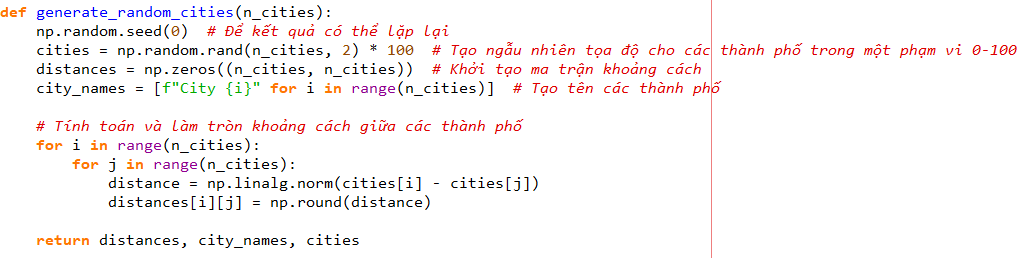
\includegraphics[width=\textwidth]{./Image/Hàm khởi tạo thành phố và khoảng cách.png}
		\caption{Hàm khởi tạo thành phố và khoảng cách}
		\label{fig:mylabel}
	\end{figure}
	
	\subsubsection{Thuật toán Di truyền (Genetic Algorithms - GA)}
	\textbf{Code:}
	\begin{center}
		\begin{figure}[htbp]
		 		\centering
		 		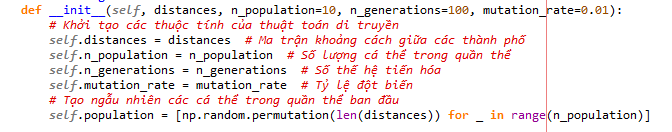
\includegraphics[width=\textwidth]{./Image/Hàm khởi tạo GA.png}
		 		\caption{Hàm khởi tạo}
		 		\label{fig:mylabel}
		 	\end{figure}
	 	\begin{figure}[htbp]
		 		\centering
		 		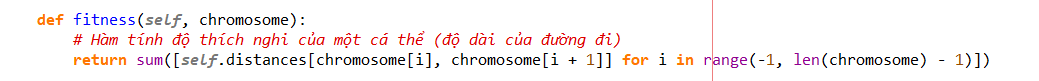
\includegraphics[width=\textwidth]{./Image/Hàm thích nghi GA.png}
		 		\caption{Hàm thích nghi}
		 		\label{fig:mylabel}
		 	\end{figure}
	 	\begin{figure}[htbp]
		 		\centering
		 		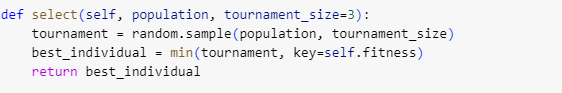
\includegraphics[width=\textwidth]{./Image/Hàm chọn GA.png}
		 		\caption{Hàm lựa chọn}
		 		\label{fig:mylabel}
		 	\end{figure}
	 	\begin{figure}[htbp]
		 		\centering
		 		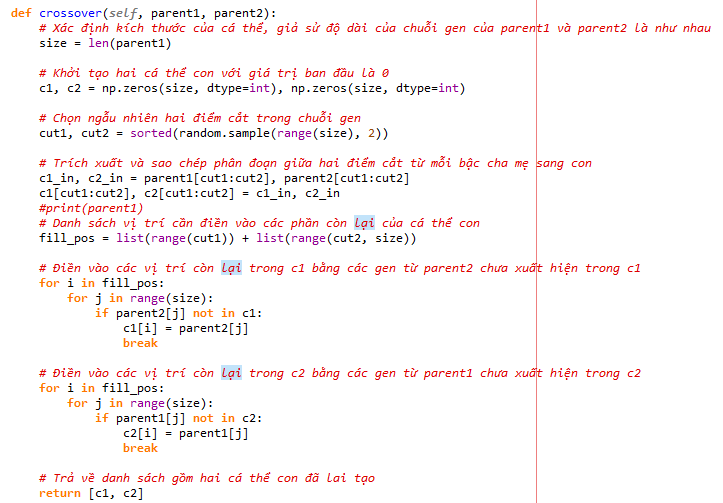
\includegraphics[width=\textwidth]{./Image/Hàm lai chéo GA.png}
		 		\caption{Hàm lai chéo}
		 		\label{fig:mylabel}
		 	\end{figure}
	 	\begin{figure}[htbp]
		 		\centering
		 		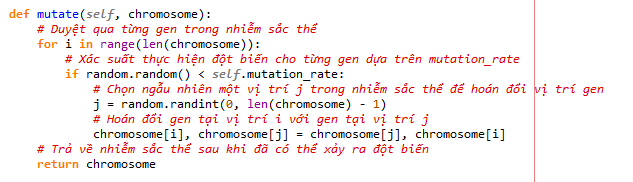
\includegraphics[width=\textwidth]{./Image/Hàm đột biến GA.png}
		 		\caption{Hàm đột biến}
		 		\label{fig:mylabel}
		 	\end{figure}
	 	\begin{figure}[htbp]
	 		\centering
	 		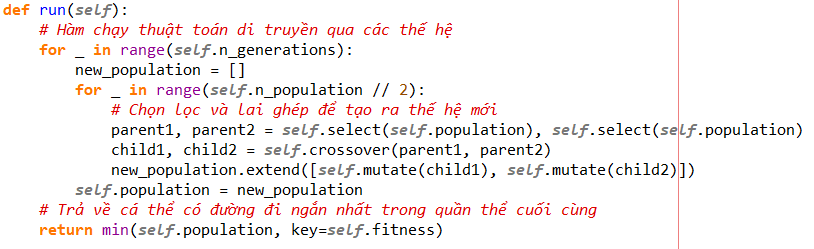
\includegraphics[width=\textwidth]{./Image/Hàm khởi chạy GA.png}
	 		\caption{Hàm khởi chạy}
	 		\label{fig:mylabel}
	 	\end{figure}
	\end{center}

	\newpage
	\textbf{Kết quả với 10 thành phố:}
	\begin{itemize}
	 	\item Best route: [9, 6, 3, 8, 7, 4, 5, 1, 2, 0]
	 	\item Best distance: 351.0
	 	\item Execution time: 0.18 seconds
	\end{itemize}
	\begin{figure}[htbp]
		\centering
		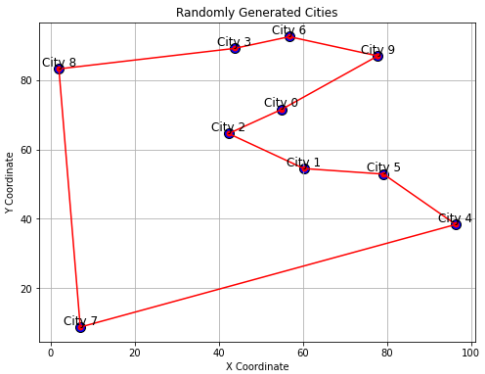
\includegraphics[width=0.7\textwidth]{./Image/GA 10 city.png}
		\caption{Dường đi khi sử dụng GA}
		\label{fig:mylabel}
	\end{figure}
	\newpage
	\textbf{Kết quả sau khi thay đổi các thuộc tính}
	\begin{center}
	 	\begin{figure}[htbp]
	 		\centering
	 		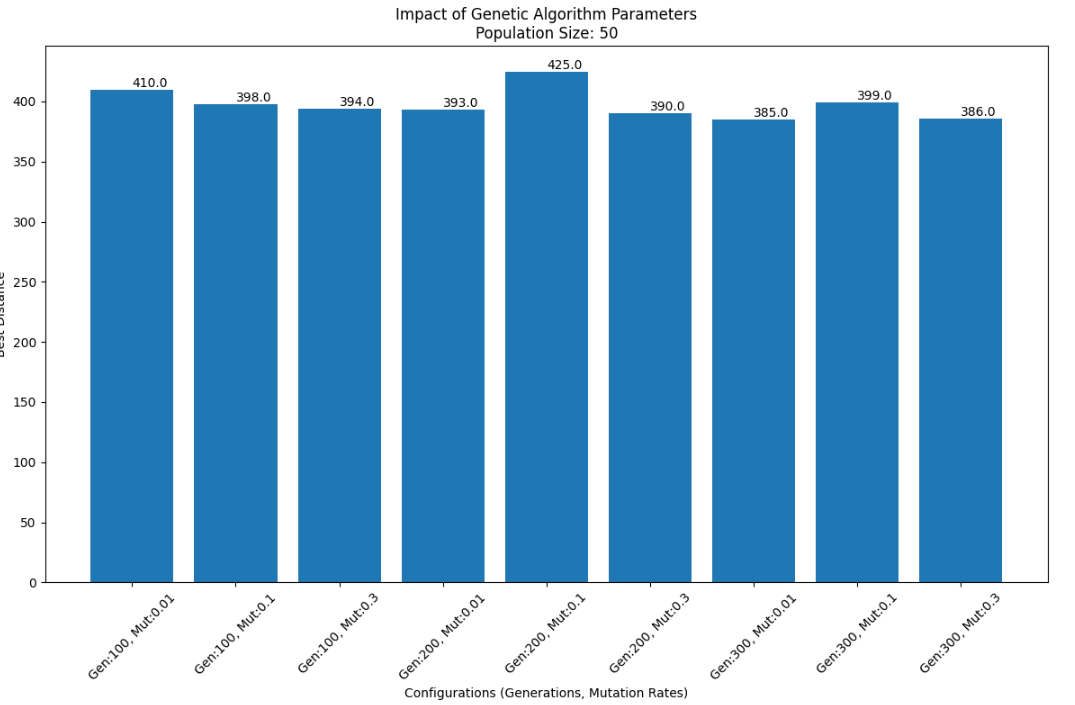
\includegraphics[width=\textwidth]{./Image/population_size_50.png}
	 		\caption{Kích thước quần thể: 50}
	 		\label{fig:mylabel}
	 	\end{figure}
	 	\begin{figure}[htbp]
	 		\centering
	 		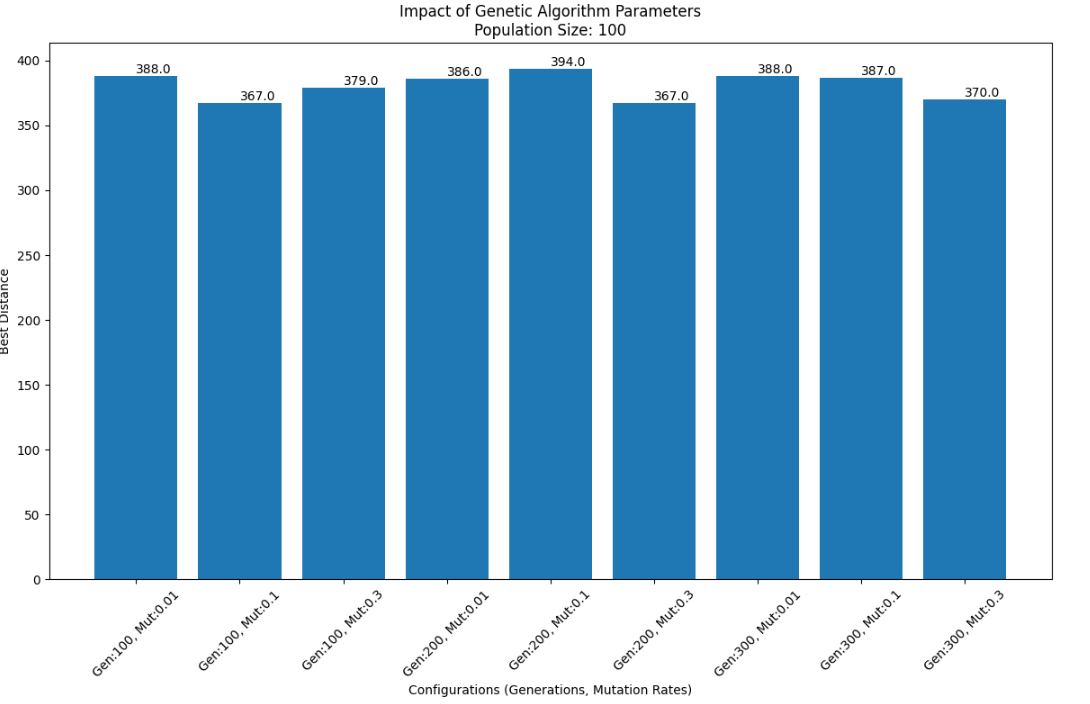
\includegraphics[width=0.8\textwidth]{./Image/population_size_100.png}
	 		\caption{Kích thước quần thể: 100}
	 		\label{fig:mylabel}
	 	\end{figure}
		 \begin{figure}[htbp]
		 	\centering
		 	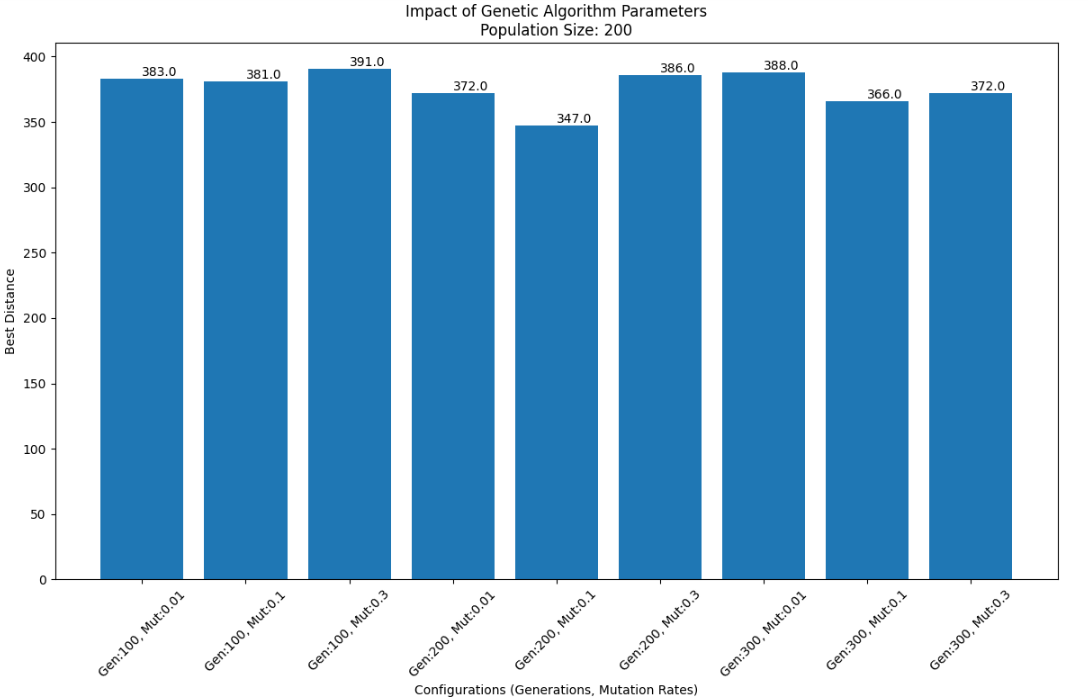
\includegraphics[width=0.8\textwidth]{./Image/population_size_200.png}
		 	\caption{Kích thước quần thể: 200}
		 	\label{fig:mylabel}
		 \end{figure}
	\end{center}
	\newpage
	\subsubsection{Thuật toán tối ưu hóa đàn kiến (Ant Colony Optimization - ACO)}
	\textbf{Code:}
	\begin{center}
		\begin{figure}[htbp]
			\centering
			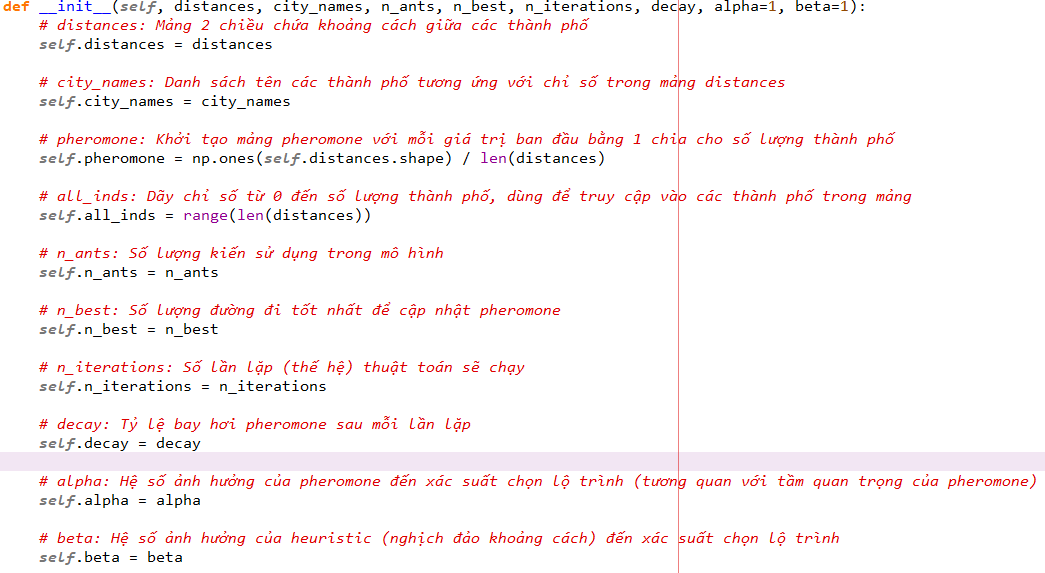
\includegraphics[width=\textwidth]{./Image/Hàm khởi tạo ACO.png}
			\caption{Hàm khởi tạo thuật toán}
			\label{fig:mylabel}
		\end{figure}
		\begin{figure}[htbp]
			\centering
			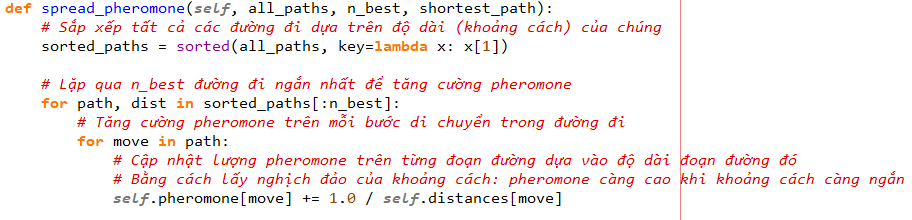
\includegraphics[width=\textwidth]{./Image/Hàm cập nhật pheromone ACO.png}
			\caption{Hàm cập nhật pheromone cho các đường đi}
			\label{fig:mylabel}
		\end{figure}
		\begin{figure}[htbp]
			\centering
			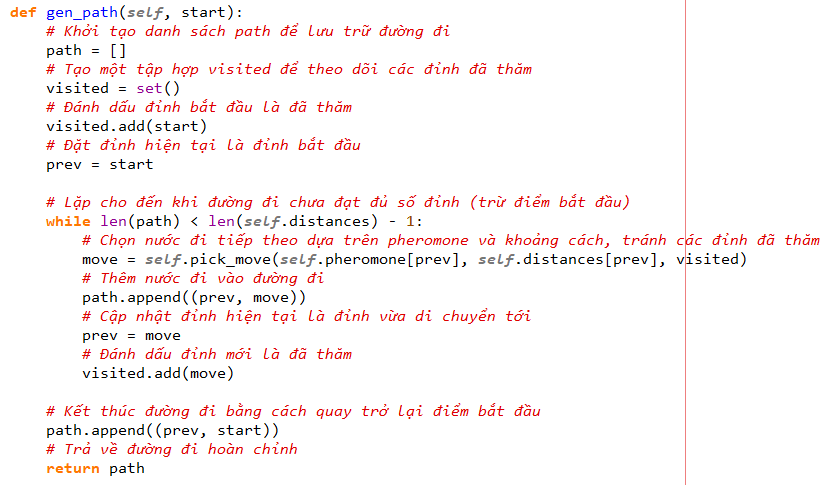
\includegraphics[width=\textwidth]{./Image/Hàm lưu lại đường đi ACO.png}
			\caption{Hàm sinh ra đường đi}
			\label{fig:mylabel}
		\end{figure}
		\begin{figure}[htbp]
			\centering
			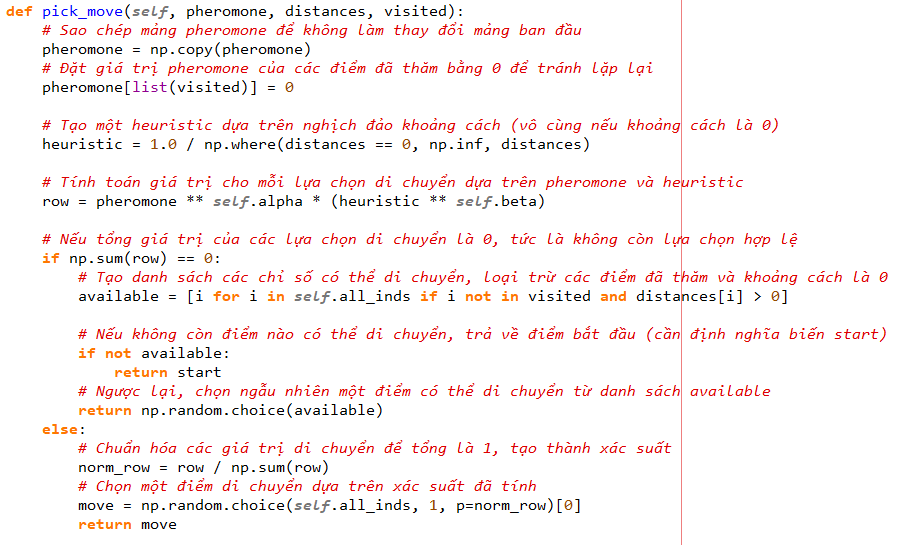
\includegraphics[width=\textwidth]{./Image/Hàm kiến di chuyển ACO.png}
			\caption{Hàm di chuyển cho kiến}
			\label{fig:mylabel}
		\end{figure}
		\begin{figure}[htbp]
			\centering
			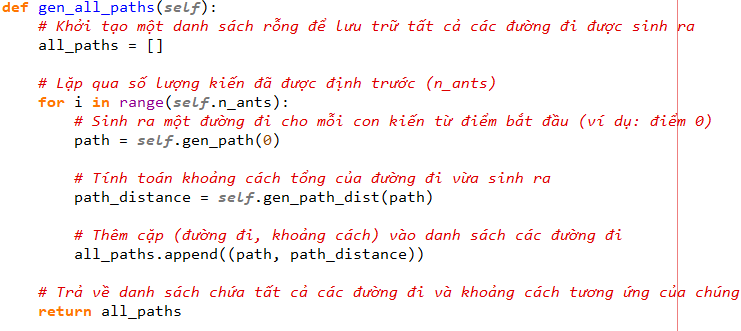
\includegraphics[width=\textwidth]{./Image/Hàm sinh ra tất cả các đường ACO.png}
			\caption{Hàm sinh ra tất cả đường đi}
			\label{fig:mylabel}
		\end{figure}
		\begin{figure}[htbp]
			\centering
			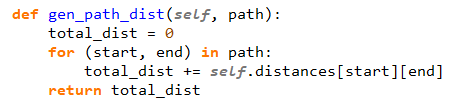
\includegraphics[width=0.8\textwidth]{./Image/Hàm tính quãng đường ACO.png}
			\caption{hàm tính quãng đường}
			\label{fig:mylabel}
		\end{figure}
		\begin{figure}[htbp]
			\centering
			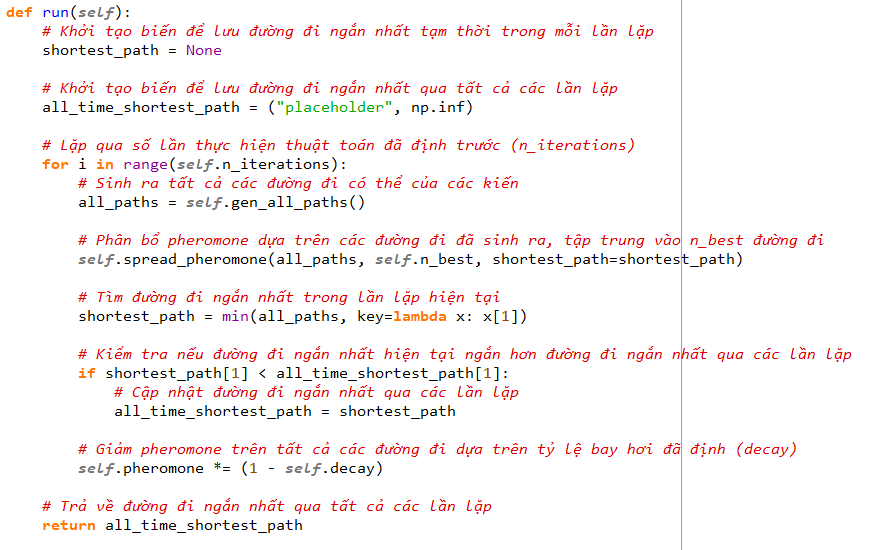
\includegraphics[width=\textwidth]{./Image/Hàm chạy ACO.png}
			\caption{Hàm chạy thuật toán}
			\label{fig:mylabel}
		\end{figure}
	\end{center}

	\newpage
	\textbf{Kết quả với 10 thành phố:}
	\begin{itemize}
	 	\item Shortest path: [(0, 2), (2, 7), (7, 8), (8, 3), (3, 6), (6, 9), (9, 5), (5, 4), (4, 1), (1, 0)]
	 	\item Best distance: 347.0
	 	\item Execution time: 0.96 seconds
	\end{itemize}
	\begin{figure}[htbp]
		\centering
		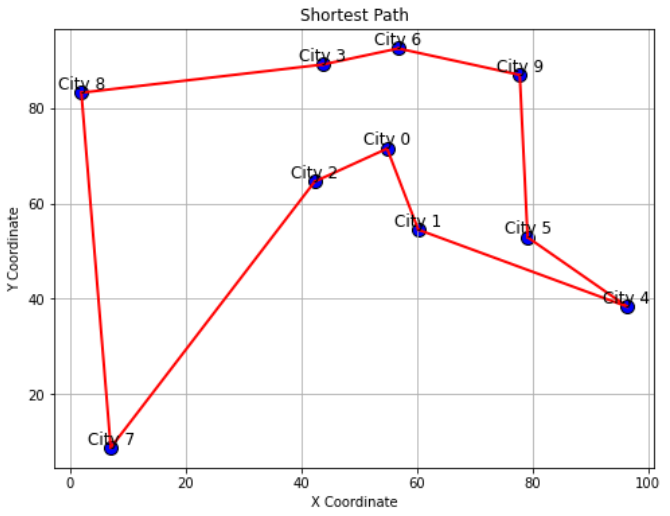
\includegraphics[width=\textwidth]{./Image/ACO 10 city.png}
		\caption{Đường di khi sử dụng ACO}
		\label{fig:mylabel}
	\end{figure}

	\newpage
	\textbf{Kết quả sau khi thay đổi các thuộc tính}
	\begin{center}
		\begin{figure}[htbp]
			\centering
			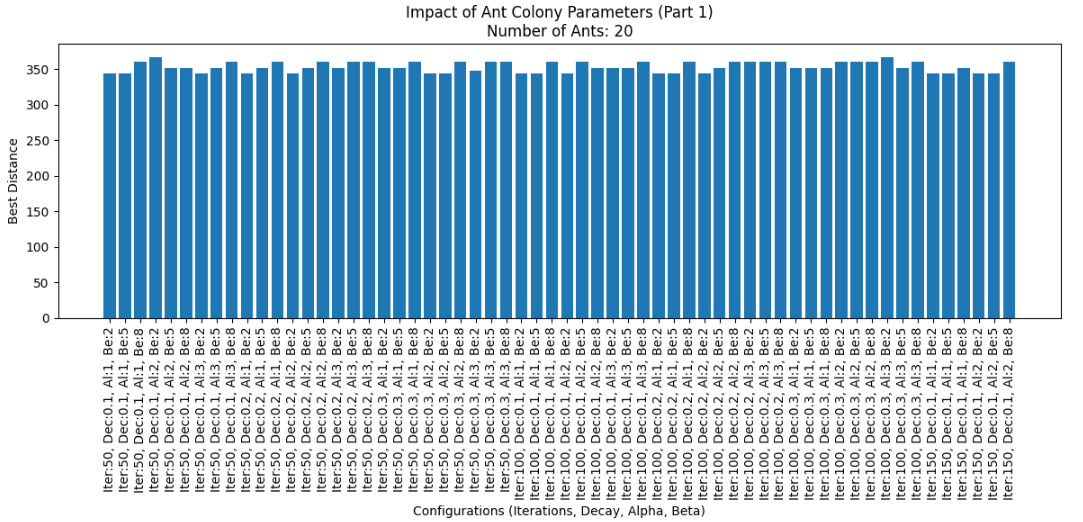
\includegraphics[width=\textwidth]{./Image/20_part1.png}
			\caption{Số kiến 20 part 1}
			\label{fig:mylabel}
		\end{figure}
	
		\begin{figure}[htbp]
			\centering
			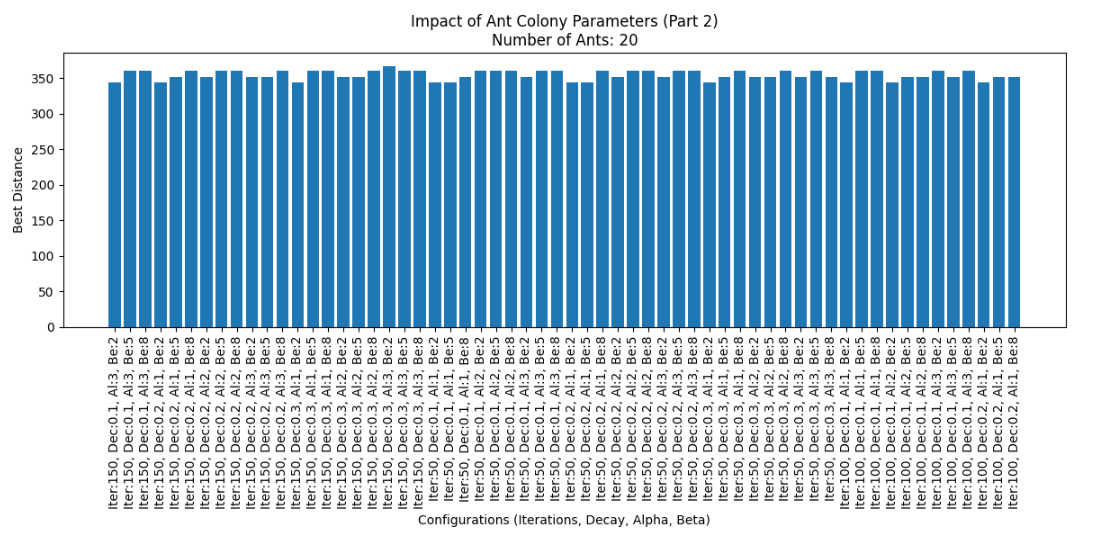
\includegraphics[width=0.8\textwidth]{./Image/20_part2.png}
			\caption{Số kiến 20 part 2}
			\label{fig:mylabel}
		\end{figure}
	
		\begin{figure}[htbp]
			\centering
			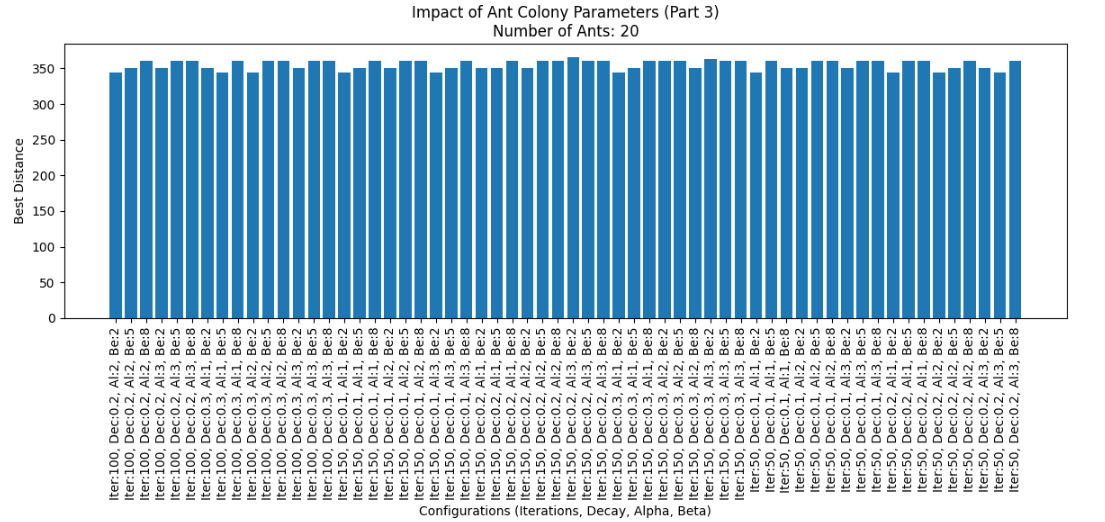
\includegraphics[width=\textwidth]{./Image/20_part3.png}
			\caption{Số kiến 20 part 3}
			\label{fig:mylabel}
		\end{figure}
		\begin{figure}[htbp]
			\centering
			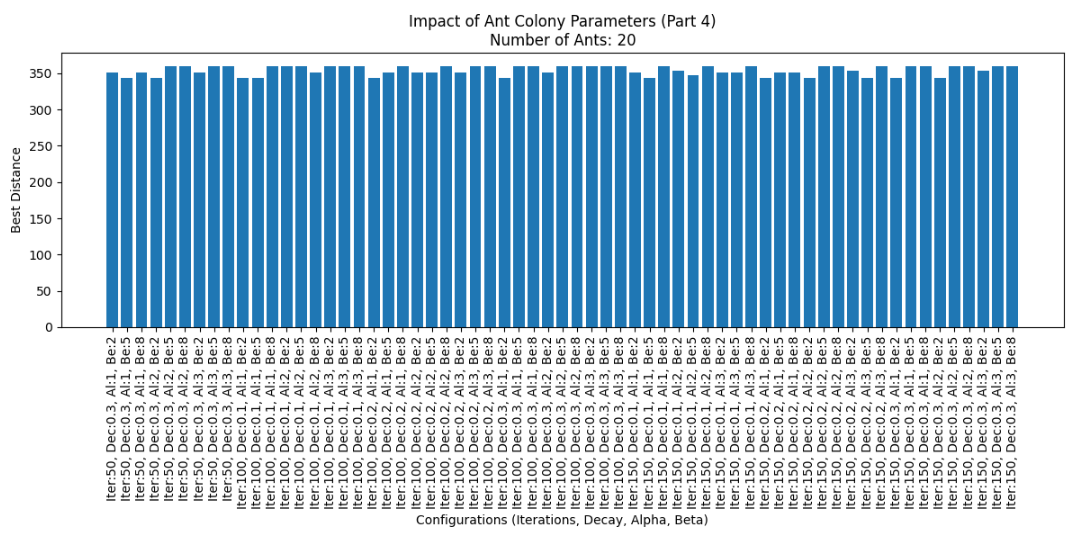
\includegraphics[width=\textwidth]{./Image/20_part4.png}
			\caption{Số kiến 20 part 4}
			\label{fig:mylabel}
		\end{figure}
		\begin{figure}[htbp]
			\centering
			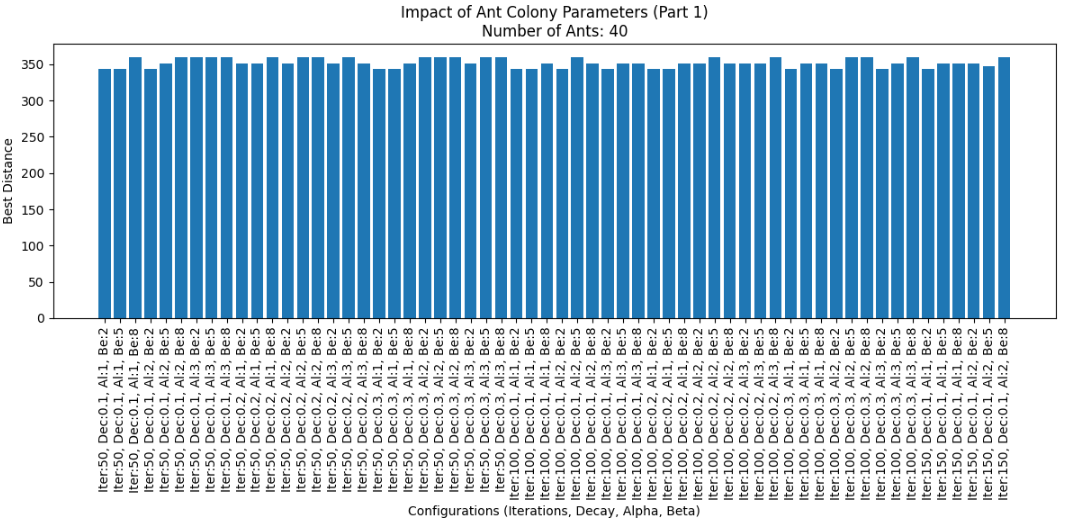
\includegraphics[width=\textwidth]{./Image/40_part1.png}
			\caption{Số kiến 40 part 1}
			\label{fig:mylabel}
		\end{figure}
		
		\begin{figure}[htbp]
			\centering
			\includegraphics[width=\textwidth]{./Image/40_part2.png}
			\caption{Số kiến 40 part 2}
			\label{fig:mylabel}
		\end{figure}
		
		\begin{figure}[htbp]
			\centering
			\includegraphics[width=\textwidth]{./Image/40_part3.png}
			\caption{Số kiến 40 part 3}
			\label{fig:mylabel}
		\end{figure}
		\begin{figure}[htbp]
			\centering
			\includegraphics[width=\textwidth]{./Image/40_part4.png}
			\caption{Số kiến 40 part 4}
			\label{fig:mylabel}
		\end{figure}
		\begin{figure}[htbp]
			\centering
			\includegraphics[width=\textwidth]{./Image/60_part1.png}
			\caption{Số kiến 60 part 1}
			\label{fig:mylabel}
		\end{figure}
		
		\begin{figure}[htbp]
			\centering
			\includegraphics[width=\textwidth]{./Image/60_part2.png}
			\caption{Số kiến 60 part 2}
			\label{fig:mylabel}
		\end{figure}
		
		\begin{figure}[htbp]
			\centering
			\includegraphics[width=\textwidth]{./Image/60_part3.png}
			\caption{Số kiến 60 part 3}
			\label{fig:mylabel}
		\end{figure}
		\begin{figure}[htbp]
			\centering
			\includegraphics[width=\textwidth]{./Image/60_part4.png}
			\caption{Số kiến 60 part 4}
			\label{fig:mylabel}
		\end{figure}
	\end{center}
	\newpage
	\subsection{Kết quả}
	\textbf{Hiệu suất:}
	\begin{center}
		\begin{figure}[htbp]
			\centering
			\includegraphics[width=0.9\textwidth]{./Image/Hiệu suất GA.png}
			\caption{Hiệu suất của thuật toán di truyền}
			\label{fig:mylabel}
		\end{figure}
		\begin{figure}[htbp]
			\centering
			\includegraphics[width=0.9\textwidth]{./Image/Hiệu suất ACO.png}
			\caption{Hiệu suất của thuật toán tối ưu hóa đàn kiến}
			\label{fig:mylabel}
		\end{figure}
		\begin{figure}[htbp]
			\centering
			\includegraphics[width=0.9\textwidth]{./Image/Hiệu suất Greendy.png}
			\caption{Hiệu suất của thuật toán tham lam}
			\label{fig:mylabel}
		\end{figure}
	\end{center}

	\newpage
	\section{ Kết luận, đánh giá và nhận xét}
	
	\subsection{Nhận xét}
	\begin{itemize}
		\item Cả ACO và GA đều là những công cụ mạnh mẽ và có những ưu điểm riêng biệt phù hợp với các loại bài toán khác nhau. ACO thường được ưu tiên khi cần một giải pháp tối ưu chính xác cho các bài toán đường đi phức tạp, trong khi GA là lựa chọn tốt cho các bài toán đòi hỏi khả năng khám phá không gian lớn và tính đa dạng cao. Việc lựa chọn giữa hai thuật toán phụ thuộc vào đặc điểm cụ thể của từng bài toán và mục tiêu tối ưu hóa.
		\item Với kết quả trên thì ta thấy được so sánh thuật toán tham lam (Greedy) với 2 thuật toán GA và ACO thì ACO là 1 thuật toán tìm đường mạnh mẽ, có thể tìm thấy con đường tối ưu hơn cả Greedy mặc dù thời gian mà ACO tìm đường lâu hơn với 2 thuật toán còn lại nhưng lại tối ưu hóa hơn hẳn về kết quả. Còn với GA thì thuật toán này nó chưa hẳn tối ưu vì code hiện tại đang là code của thuật toán cổ điển, cùng với đó là kết quả cũng là sự lai tạo ngẫu nhiên của các cả thể. Cho nên thuật toán sẽ bị kém hơn về mặt kết quả nhưng tốc độ ra kết quả thì nhanh hơn ACO. Nhưng đó chỉ là kết quả với 1 số liệu thuộc tính cố định vì GA có kết quả còn dựa theo vào số liệu mà người lập trình đưa vào. Vậy GA sẽ có kết quả tốt khi thực hiện nhiều lần với các quần thể ngẫu nhiên.
	\end{itemize}
	\newpage
	\subsection{Đánh giá hiệu quả}
	\paragraph{Thuật toán Di truyền (GA)}
	\begin{itemize}
	 	\item \textbf{Ưu điểm:} GA tốt trong việc tìm kiếm trên không gian lớn và có khả năng thoát khỏi các điểm tối ưu cục bộ nhờ vào cơ chế đột biến và lai ghép.
	 	\item \textbf{Nhược điểm:} Kết quả tối ưu phụ thuộc nhiều vào các tham số như tỷ lệ đột biến và cách thức lai ghép. Đôi khi, việc tinh chỉnh các tham số này để đạt hiệu quả tối ưu có thể rất phức tạp và mất rất nhiều thời gian.
	\end{itemize}
	
	\paragraph{Thuật toán kiến (ACO)}
	\begin{itemize}
	 	\item \textbf{Ưu điểm:} ACO rất mạnh trong việc tìm kiếm đường đi dựa trên cơ chế pheromone, cho phép chia sẻ thông tin giữa các cá thể, từ đó hướng tới giải pháp tốt chung.
	 	\item \textbf{Nhược điểm:} ACO có thể mất nhiều thời gian hơn để hội tụ, đặc biệt là khi kích thước bài toán lớn, do nó phụ thuộc vào sự phân bố pheromone và cần nhiều vòng lặp để điều chỉnh pheromone đạt được mức tối ưu.
	\end{itemize}
	
	\subsection{Độ phức tạp và thời gian thực thi}
	\paragraph{GA:}
	\begin{itemize}
		\item \textbf{Độ phức tạp:} GA thường đơn giản hơn ACO về mặt quản lý trạng thái, vì nó chỉ cần xử lý các cá thể trong quần thể thông qua các toán tử di truyền như lai ghép, đột biến và chọn lọc.
		\item \textbf{Thời gian thực thi:} GA có thể nhanh hơn ACO do khả năng song song hóa trong đánh giá độ thích nghi của quần thể, và không yêu cầu bất kỳ cập nhật trạng thái phức tạp nào giữa các thế hệ.
	\end{itemize}

	\paragraph{ACO:}
	\begin{itemize}
	 	\item \textbf{Độ phức tạp:} ACO phải xử lý và cập nhật mức pheromone trên một lưới phức tạp của các đường đi, làm tăng độ phức tạp về mặt tính toán, đặc biệt khi số lượng đường đi và điểm (nút) trong đồ thị tăng lên.
	 	\item \textbf{Thời gian thực thi:} Thời gian thực thi của ACO có thể chậm do yêu cầu cập nhật pheromone liên tục và cần nhiều lần lặp để hội tụ đến lộ trình tối ưu, đặc biệt trong các bài toán lớn và phức tạp.
	\end{itemize}
	

	\subsection{Tính năng động và khả năng thích ứng}
	
	\paragraph{GA:}
	\begin{itemize}
		\item \textbf{Tính năng động:} GA cũng có khả năng thích ứng tốt với sự thay đổi của bài toán nhờ vào độ đa dạng của quần thể, giúp nó tránh bị mắc kẹt ở tối ưu cục bộ.
		\item \textbf{Thích ứng:} GA linh hoạt hơn và có thể được áp dụng cho nhiều loại bài toán tối ưu hóa khác nhau, từ tối ưu hóa tham số đến thiết kế cấu trúc.
	\end{itemize}

	\paragraph{ACO:}
	\begin{itemize}
		\item \textbf{Tính năng động:} ACO có khả năng thích ứng cao với các thay đổi trong môi trường hoặc bài toán, nhờ vào việc pheromone được cập nhật dựa trên hiệu quả của các lộ trình được kiến khám phá.
		\item \textbf{Thích ứng:} ACO thích hợp cho các bài toán đòi hỏi việc khám phá và tối ưu hóa dựa trên các mối liên kết địa lý và đường đi phức tạp.
	\end{itemize}
	

	
	\subsection{Tính ổn định}
	\begin{itemize}
		\item \textbf{ACO:} ACO có thể ổn định nếu các tham số pheromone được cài đặt và quản lý một cách cẩn thận. Sự ổn định này tăng lên khi lượng pheromone trên các lộ trình tối ưu dần được tăng cường qua các lần lặp.
	\end{itemize}
	
	
	\begin{itemize}
		\item \textbf{GA:} có thể kém ổn định hơn do bản chất ngẫu nhiên của các toán tử di truyền, nhưng điều này cũng làm cho nó có khả năng khám phá không gian giải pháp một cách rộng rãi và đa dạng, giúp cải thiện khả năng thích ứng của thuật toán.
	\end{itemize}
	\newpage
	\section{Tài liệu tham khảo}
	\begin{thebibliography}{99} % Số 99 chỉ là giới hạn tối đa của danh sách, có thể thay đổi nếu bạn có nhiều tài liệu hơn
		
		\bibitem{tinHoc3} Tài liệu chuyên tin học quyển 3.
		\bibitem{geeksGA} \url{https://www.geeksforgeeks.org/genetic-algorithms/?ref=header_search}
		\bibitem{encodingGA} \url{https://www.geeksforgeeks.org/encoding-methods-in-genetic-algorithm/?ref=header_search}
		\bibitem{projectIdeaGA} \url{https://www.geeksforgeeks.org/project-idea-genetic-algorithms-for-graph-colouring/?ref=header_search}
		\bibitem{sciendo} \url{https://intapi.sciendo.com/pdf/10.2478/v10238-012-0039-2}
		\bibitem{corePDF} \url{https://core.ac.uk/download/pdf/32452919.pdf}
		\bibitem{linkedinGA} \url{https://www.linkedin.com/pulse/use-genetic-algorithms-planning-scheduling-projects-well-suleiman}
		\bibitem{nerophung} \url{https://nerophung.github.io/2020/05/28/genetic-algorithm#thu%E1%BA%ADt-to%C3%A1n-di-truy%E1%BB%81n}
		\bibitem{datadrivenGA} \url{https://medium.datadriveninvestor.com/genetic-algorithm-made-intuitive-with-natural-selection-and-python-project-from-scratch-3462f7793a3f}
		\bibitem{youtubeGA1} \url{https://www.youtube.com/watch?v=fxCHAkYAjis&list=PLALZwazFybKKeKPXDP4EjrDLNW436xiLI&index=2}
		\bibitem{youtubeGA2} \url{https://www.youtube.com/watch?v=MGY3Vf_M4Qs}
		\bibitem{towardsDSGA1} \url{https://towardsdatascience.com/introduction-to-genetic-algorithms-including-example-code-e396e98d8bf3}
		\bibitem{geeksACO1} \url{https://www.geeksforgeeks.org/introduction-to-ant-colony-optimization/}
		\bibitem{geeksACO2} \url{https://www.geeksforgeeks.org/introduction-to-ant-colony-optimization/?ref=header_search}
		\bibitem{towardsDSGA2} \url{https://towardsdatascience.com/introduction-to-genetic-algorithms-including-example-code-e396e98d8bf3}
		\bibitem{steadyGA} \url{https://www.geeksforgeeks.org/steady-state-genetic-algorithm-ssga/}
		\bibitem{sciDirect} \url{https://www.sciencedirect.com/science/article/abs/pii/S0377221705009367}
		\bibitem{researchgateSched} \url{https://www.researchgate.net/publication/235683206_Simultaneous_scheduling_of_production_and_maintenance_tasks_in_the_job_shop}
		\bibitem{altairHelp} \url{https://2021.help.altair.com/2021/hwdesktop/hst/topics/design_exploration/method_multi_objective_genetirc_algorithm_r.htm}
		\bibitem{researchMurata} \url{https://www.inf.unioeste.br/~adair/MOA/Artigos/MO/MOGA%20-%20Multiobjective%20GA%20-%20Murata%20Ishibuchi.pdf}
		\bibitem{researchgateAdaptive} \url{https://www.researchgate.net/figure/The-flowchart-of-adaptive-genetic-algorithm_fig4_322397724}
		\bibitem{intechOpen} \url{https://www.intechopen.com/chapters/81745}
		\bibitem{researchgateParallel} \url{https://www.researchgate.net/publication/339969145_An_OpenMP_Parallel_Genetic_Algorithm_for_Design_Space_Exploration_of_Heterogeneous_Multi-processor_Embedded_Systems}
		\bibitem{researchAntenna} \url{https://www.researchgate.net/publication/44247443_Exploiting_of_the_Compression_Methods_for_Reconstruction_of_the_Antenna_Far-Field_Using_Only_Amplitude_Near-Field_Measurements}
		\bibitem{arxivPaper} \url{https://arxiv.org/pdf/1610.00976}
		\bibitem{acsEC97} \url{https://people.idsia.ch/~luca/acs-ec97.pdf}
		\bibitem{sciDirectMO} \url{https://www.sciencedirect.com/science/article/abs/pii/S1568494612001901}
		\bibitem{sciDirectRecent} \url{https://www.sciencedirect.com/science/article/abs/pii/S0950705121011102}
		\bibitem{researchgateScheduling} \url{https://www.researchgate.net/publication/337700129_Q-learning_and_ACO_hybridisation_for_real-time_scheduling_on_heterogeneous_distributed_architectures}
		\bibitem{mdpiAP} \url{https://www.mdpi.com/2076-3417/12/21/11219}
		\bibitem{mdpiAlgorithms} \url{https://www.mdpi.com/1999-4893/14/10/286}
		\bibitem{researchHyperCube} \url{https://www.researchgate.net/publication/8337732_The_Hyper-Cube_Framework_for_Ant_Colony_Optimization}
		
	\end{thebibliography}
	
\end{document}
